
%% bare_jrnl.tex
%% V1.4b
%% 2015/08/26
%% by Michael Shell
%% see http://www.michaelshell.org/
%% for current contact information.
%%
%% This is a skeleton file demonstrating the use of IEEEtran.cls
%% (requires IEEEtran.cls version 1.8b or later) with an IEEE
%% journal paper.
%%
%% Support sites:
%% http://www.michaelshell.org/tex/ieeetran/
%% http://www.ctan.org/pkg/ieeetran
%% and
%% http://www.ieee.org/

%%*************************************************************************
%% Legal Notice:
%% This code is offered as-is without any warranty either expressed or
%% implied; without even the implied warranty of MERCHANTABILITY or
%% FITNESS FOR A PARTICULAR PURPOSE! 
%% User assumes all risk.
%% In no event shall the IEEE or any contributor to this code be liable for
%% any damages or losses, including, but not limited to, incidental,
%% consequential, or any other damages, resulting from the use or misuse
%% of any information contained here.
%%
%% All comments are the opinions of their respective authors and are not
%% necessarily endorsed by the IEEE.
%%
%% This work is distributed under the LaTeX Project Public License (LPPL)
%% ( http://www.latex-project.org/ ) version 1.3, and may be freely used,
%% distributed and modified. A copy of the LPPL, version 1.3, is included
%% in the base LaTeX documentation of all distributions of LaTeX released
%% 2003/12/01 or later.
%% Retain all contribution notices and credits.
%% ** Modified files should be clearly indicated as such, including  **
%% ** renaming them and changing author support contact information. **
%%*************************************************************************


% *** Authors should verify (and, if needed, correct) their LaTeX system  ***
% *** with the testflow diagnostic prior to trusting their LaTeX platform ***
% *** with production work. The IEEE's font choices and paper sizes can   ***
% *** trigger bugs that do not appear when using other class files.       ***                          ***
% The testflow support page is at:
% http://www.michaelshell.org/tex/testflow/



\documentclass[journal]{IEEEtran}
%
% If IEEEtran.cls has not been installed into the LaTeX system files,
% manually specify the path to it like:
% \documentclass[journal]{../sty/IEEEtran}


\usepackage[utf8]{inputenc}
\usepackage{graphicx}
\usepackage{subcaption} 
\usepackage{hyperref}
\usepackage{algorithm2e} % For algorithms
\usepackage{amsmath, amssymb, amsthm} % Mathematical packages


% Some very useful LaTeX packages include:
% (uncomment the ones you want to load)


% *** MISC UTILITY PACKAGES ***
%
%\usepackage{ifpdf}
% Heiko Oberdiek's ifpdf.sty is very useful if you need conditional
% compilation based on whether the output is pdf or dvi.
% usage:
% \ifpdf
%   % pdf code
% \else
%   % dvi code
% \fi
% The latest version of ifpdf.sty can be obtained from:
% http://www.ctan.org/pkg/ifpdf
% Also, note that IEEEtran.cls V1.7 and later provides a builtin
% \ifCLASSINFOpdf conditional that works the same way.
% When switching from latex to pdflatex and vice-versa, the compiler may
% have to be run twice to clear warning/error messages.






% *** CITATION PACKAGES ***
%
%\usepackage{cite}
% cite.sty was written by Donald Arseneau
% V1.6 and later of IEEEtran pre-defines the format of the cite.sty package
% \cite{} output to follow that of the IEEE. Loading the cite package will
% result in citation numbers being automatically sorted and properly
% "compressed/ranged". e.g., [1], [9], [2], [7], [5], [6] without using
% cite.sty will become [1], [2], [5]--[7], [9] using cite.sty. cite.sty's
% \cite will automatically add leading space, if needed. Use cite.sty's
% noadjust option (cite.sty V3.8 and later) if you want to turn this off
% such as if a citation ever needs to be enclosed in parenthesis.
% cite.sty is already installed on most LaTeX systems. Be sure and use
% version 5.0 (2009-03-20) and later if using hyperref.sty.
% The latest version can be obtained at:
% http://www.ctan.org/pkg/cite
% The documentation is contained in the cite.sty file itself.






% *** GRAPHICS RELATED PACKAGES ***
%
\ifCLASSINFOpdf
  % \usepackage[pdftex]{graphicx}
  % declare the path(s) where your graphic files are
  % \graphicspath{{../pdf/}{../jpeg/}}
  % and their extensions so you won't have to specify these with
  % every instance of \includegraphics
  % \DeclareGraphicsExtensions{.pdf,.jpeg,.png}
\else
  % or other class option (dvipsone, dvipdf, if not using dvips). graphicx
  % will default to the driver specified in the system graphics.cfg if no
  % driver is specified.
  % \usepackage[dvips]{graphicx}
  % declare the path(s) where your graphic files are
  % \graphicspath{{../eps/}}
  % and their extensions so you won't have to specify these with
  % every instance of \includegraphics
  % \DeclareGraphicsExtensions{.eps}
\fi
% graphicx was written by David Carlisle and Sebastian Rahtz. It is
% required if you want graphics, photos, etc. graphicx.sty is already
% installed on most LaTeX systems. The latest version and documentation
% can be obtained at: 
% http://www.ctan.org/pkg/graphicx
% Another good source of documentation is "Using Imported Graphics in
% LaTeX2e" by Keith Reckdahl which can be found at:
% http://www.ctan.org/pkg/epslatex
%
% latex, and pdflatex in dvi mode, support graphics in encapsulated
% postscript (.eps) format. pdflatex in pdf mode supports graphics
% in .pdf, .jpeg, .png and .mps (metapost) formats. Users should ensure
% that all non-photo figures use a vector format (.eps, .pdf, .mps) and
% not a bitmapped formats (.jpeg, .png). The IEEE frowns on bitmapped formats
% which can result in "jaggedy"/blurry rendering of lines and letters as
% well as large increases in file sizes.
%
% You can find documentation about the pdfTeX application at:
% http://www.tug.org/applications/pdftex





% *** MATH PACKAGES ***
%
%\usepackage{amsmath}
% A popular package from the American Mathematical Society that provides
% many useful and powerful commands for dealing with mathematics.
%
% Note that the amsmath package sets \interdisplaylinepenalty to 10000
% thus preventing page breaks from occurring within multiline equations. Use:
%\interdisplaylinepenalty=2500
% after loading amsmath to restore such page breaks as IEEEtran.cls normally
% does. amsmath.sty is already installed on most LaTeX systems. The latest
% version and documentation can be obtained at:
% http://www.ctan.org/pkg/amsmath





% *** SPECIALIZED LIST PACKAGES ***
%
%\usepackage{algorithmic}
% algorithmic.sty was written by Peter Williams and Rogerio Brito.
% This package provides an algorithmic environment fo describing algorithms.
% You can use the algorithmic environment in-text or within a figure
% environment to provide for a floating algorithm. Do NOT use the algorithm
% floating environment provided by algorithm.sty (by the same authors) or
% algorithm2e.sty (by Christophe Fiorio) as the IEEE does not use dedicated
% algorithm float types and packages that provide these will not provide
% correct IEEE style captions. The latest version and documentation of
% algorithmic.sty can be obtained at:
% http://www.ctan.org/pkg/algorithms
% Also of interest may be the (relatively newer and more customizable)
% algorithmicx.sty package by Szasz Janos:
% http://www.ctan.org/pkg/algorithmicx




% *** ALIGNMENT PACKAGES ***
%
%\usepackage{array}
% Frank Mittelbach's and David Carlisle's array.sty patches and improves
% the standard LaTeX2e array and tabular environments to provide better
% appearance and additional user controls. As the default LaTeX2e table
% generation code is lacking to the point of almost being broken with
% respect to the quality of the end results, all users are strongly
% advised to use an enhanced (at the very least that provided by array.sty)
% set of table tools. array.sty is already installed on most systems. The
% latest version and documentation can be obtained at:
% http://www.ctan.org/pkg/array


% IEEEtran contains the IEEEeqnarray family of commands that can be used to
% generate multiline equations as well as matrices, tables, etc., of high
% quality.




% *** SUBFIGURE PACKAGES ***
%\ifCLASSOPTIONcompsoc
%  \usepackage[caption=false,font=normalsize,labelfont=sf,textfont=sf]{subfig}
%\else
%  \usepackage[caption=false,font=footnotesize]{subfig}
%\fi
% subfig.sty, written by Steven Douglas Cochran, is the modern replacement
% for subfigure.sty, the latter of which is no longer maintained and is
% incompatible with some LaTeX packages including fixltx2e. However,
% subfig.sty requires and automatically loads Axel Sommerfeldt's caption.sty
% which will override IEEEtran.cls' handling of captions and this will result
% in non-IEEE style figure/table captions. To prevent this problem, be sure
% and invoke subfig.sty's "caption=false" package option (available since
% subfig.sty version 1.3, 2005/06/28) as this is will preserve IEEEtran.cls
% handling of captions.
% Note that the Computer Society format requires a larger sans serif font
% than the serif footnote size font used in traditional IEEE formatting
% and thus the need to invoke different subfig.sty package options depending
% on whether compsoc mode has been enabled.
%
% The latest version and documentation of subfig.sty can be obtained at:
% http://www.ctan.org/pkg/subfig




% *** FLOAT PACKAGES ***
%
%\usepackage{fixltx2e}
% fixltx2e, the successor to the earlier fix2col.sty, was written by
% Frank Mittelbach and David Carlisle. This package corrects a few problems
% in the LaTeX2e kernel, the most notable of which is that in current
% LaTeX2e releases, the ordering of single and double column floats is not
% guaranteed to be preserved. Thus, an unpatched LaTeX2e can allow a
% single column figure to be placed prior to an earlier double column
% figure.
% Be aware that LaTeX2e kernels dated 2015 and later have fixltx2e.sty's
% corrections already built into the system in which case a warning will
% be issued if an attempt is made to load fixltx2e.sty as it is no longer
% needed.
% The latest version and documentation can be found at:
% http://www.ctan.org/pkg/fixltx2e


%\usepackage{stfloats}
% stfloats.sty was written by Sigitas Tolusis. This package gives LaTeX2e
% the ability to do double column floats at the bottom of the page as well
% as the top. (e.g., "\begin{figure*}[!b]" is not normally possible in
% LaTeX2e). It also provides a command:
%\fnbelowfloat
% to enable the placement of footnotes below bottom floats (the standard
% LaTeX2e kernel puts them above bottom floats). This is an invasive package
% which rewrites many portions of the LaTeX2e float routines. It may not work
% with other packages that modify the LaTeX2e float routines. The latest
% version and documentation can be obtained at:
% http://www.ctan.org/pkg/stfloats
% Do not use the stfloats baselinefloat ability as the IEEE does not allow
% \baselineskip to stretch. Authors submitting work to the IEEE should note
% that the IEEE rarely uses double column equations and that authors should try
% to avoid such use. Do not be tempted to use the cuted.sty or midfloat.sty
% packages (also by Sigitas Tolusis) as the IEEE does not format its papers in
% such ways.
% Do not attempt to use stfloats with fixltx2e as they are incompatible.
% Instead, use Morten Hogholm'a dblfloatfix which combines the features
% of both fixltx2e and stfloats:
%
% \usepackage{dblfloatfix}
% The latest version can be found at:
% http://www.ctan.org/pkg/dblfloatfix




%\ifCLASSOPTIONcaptionsoff
%  \usepackage[nomarkers]{endfloat}
% \let\MYoriglatexcaption\caption
% \renewcommand{\caption}[2][\relax]{\MYoriglatexcaption[#2]{#2}}
%\fi
% endfloat.sty was written by James Darrell McCauley, Jeff Goldberg and 
% Axel Sommerfeldt. This package may be useful when used in conjunction with 
% IEEEtran.cls'  captionsoff option. Some IEEE journals/societies require that
% submissions have lists of figures/tables at the end of the paper and that
% figures/tables without any captions are placed on a page by themselves at
% the end of the document. If needed, the draftcls IEEEtran class option or
% \CLASSINPUTbaselinestretch interface can be used to increase the line
% spacing as well. Be sure and use the nomarkers option of endfloat to
% prevent endfloat from "marking" where the figures would have been placed
% in the text. The two hack lines of code above are a slight modification of
% that suggested by in the endfloat docs (section 8.4.1) to ensure that
% the full captions always appear in the list of figures/tables - even if
% the user used the short optional argument of \caption[]{}.
% IEEE papers do not typically make use of \caption[]'s optional argument,
% so this should not be an issue. A similar trick can be used to disable
% captions of packages such as subfig.sty that lack options to turn off
% the subcaptions:
% For subfig.sty:
% \let\MYorigsubfloat\subfloat
% \renewcommand{\subfloat}[2][\relax]{\MYorigsubfloat[]{#2}}
% However, the above trick will not work if both optional arguments of
% the \subfloat command are used. Furthermore, there needs to be a
% description of each subfigure *somewhere* and endfloat does not add
% subfigure captions to its list of figures. Thus, the best approach is to
% avoid the use of subfigure captions (many IEEE journals avoid them anyway)
% and instead reference/explain all the subfigures within the main caption.
% The latest version of endfloat.sty and its documentation can obtained at:
% http://www.ctan.org/pkg/endfloat
%
% The IEEEtran \ifCLASSOPTIONcaptionsoff conditional can also be used
% later in the document, say, to conditionally put the References on a 
% page by themselves.




% *** PDF, URL AND HYPERLINK PACKAGES ***
%
%\usepackage{url}
% url.sty was written by Donald Arseneau. It provides better support for
% handling and breaking URLs. url.sty is already installed on most LaTeX
% systems. The latest version and documentation can be obtained at:
% http://www.ctan.org/pkg/url
% Basically, \url{my_url_here}.




% *** Do not adjust lengths that control margins, column widths, etc. ***
% *** Do not use packages that alter fonts (such as pslatex).         ***
% There should be no need to do such things with IEEEtran.cls V1.6 and later.
% (Unless specifically asked to do so by the journal or conference you plan
% to submit to, of course. )


% correct bad hyphenation here
\hyphenation{op-tical net-works semi-conduc-tor}


\begin{document}
%
% paper title
% Titles are generally capitalized except for words such as a, an, and, as,
% at, but, by, for, in, nor, of, on, or, the, to and up, which are usually
% not capitalized unless they are the first or last word of the title.
% Linebreaks \\ can be used within to get better formatting as desired.
% Do not put math or special symbols in the title.
\title{Training an Agent on Brainwaves}
%
%
% author names and IEEE memberships
% note positions of commas and nonbreaking spaces ( ~ ) LaTeX will not break
% a structure at a ~ so this keeps an author's name from being broken across
% two lines.
% use \thanks{} to gain access to the first footnote area
% a separate \thanks must be used for each paragraph as LaTeX2e's \thanks
% was not built to handle multiple paragraphs
%

\author{Bartolomé Francisco, Moreno Juan,  Navas Natalia, Vitali José, \\
Rodrigo~Ramele,~\IEEEmembership{Member,~IEEE,} 
        Juan~Miguel,~Santos% <-this % stops a space
\thanks{R. Ramele and J.M.Santos are with the Department
of Computer Engineering, Instituto Tecnológico de Buenos Aires(ITBA), Argentina,
e-mail: rramele@itba.edu.ar.}% <-this % stops a space
\thanks{Manuscript received April 19, 2005; revised August 26, 2015.}}

% note the % following the last \IEEEmembership and also \thanks - 
% these prevent an unwanted space from occurring between the last author name
% and the end of the author line. i.e., if you had this:
% 
% \author{....lastname \thanks{...} \thanks{...} }
%                     ^------------^------------^----Do not want these spaces!
%
% a space would be appended to the last name and could cause every name on that
% line to be shifted left slightly. This is one of those "LaTeX things". For
% instance, "\textbf{A} \textbf{B}" will typeset as "A B" not "AB". To get
% "AB" then you have to do: "\textbf{A}\textbf{B}"
% \thanks is no different in this regard, so shield the last } of each \thanks
% that ends a line with a % and do not let a space in before the next \thanks.
% Spaces after \IEEEmembership other than the last one are OK (and needed) as
% you are supposed to have spaces between the names. For what it is worth,
% this is a minor point as most people would not even notice if the said evil
% space somehow managed to creep in.



% The paper headers
\markboth{Journal of \LaTeX\ Class Files,~Vol.~14, No.~8, August~2015}%
{Shell \MakeLowercase{\textit{et al.}}: Bare Demo of IEEEtran.cls for IEEE Journals}
% The only time the second header will appear is for the odd numbered pages
% after the title page when using the twoside option.
% 
% *** Note that you probably will NOT want to include the author's ***
% *** name in the headers of peer review papers.                   ***
% You can use \ifCLASSOPTIONpeerreview for conditional compilation here if
% you desire.




% If you want to put a publisher's ID mark on the page you can do it like
% this:
%\IEEEpubid{0000--0000/00\$00.00~\copyright~2015 IEEE}
% Remember, if you use this you must call \IEEEpubidadjcol in the second
% column for its text to clear the IEEEpubid mark.



% use for special paper notices
%\IEEEspecialpapernotice{(Invited Paper)}




% make the title area
\maketitle

% As a general rule, do not put math, special symbols or citations
% in the abstract or keywords.
\begin{abstract}
The field of Brain Computer Interfaces has seen a bloom in the past few years. One of its applications is the training of systems using signals originated from the human brain. Out of all the methods used to acquire information from the central nervous system the one that has gained the most popularity is Electroencephalography (EEG), mainly because of its effectiveness, low cost and because it is noninvasive.
Event-related potential (ERP) are brain signals that are time-locked to a particular event. Error-related potential (ErrP) are a particular type of ERP that are can be elicited by a person who attends a recognizable error. When subjects observe an agent who makes a mistake this potential can be discerned when analyzing the signals which are directly related with the cognitive interpretation of an erroneous outcome or decision.
Reinforcement Learning (RL) is an approach to machine learning where an agent tries to maximize the reward obtained while interacting with an unknown environment. This work follow this path by detecting the ErrP potential from subjects witnessing an agent playing the game and improving the agent behavior using RL and obtaining rewards from the subjects.
\end{abstract}

% Note that keywords are not normally used for peerreview papers.
\begin{IEEEkeywords}
ErrP, BCI, EEG, RL, Agent, AI
\end{IEEEkeywords}






% For peer review papers, you can put extra information on the cover
% page as needed:
% \ifCLASSOPTIONpeerreview
% \begin{center} \bfseries EDICS Category: 3-BBND \end{center}
% \fi
%
% For peerreview papers, this IEEEtran command inserts a page break and
% creates the second title. It will be ignored for other modes.
\IEEEpeerreviewmaketitle



\section{Introduction}


% You must have at least 2 lines in the paragraph with the drop letter
% (should never be an issue)
\IEEEPARstart{T}{he} effectiveness of today's human–machine interaction and artificial intelligence is limited by a communication bottleneck as humans are required to translate high-level concepts into a machine-mandated sequence of instructions \cite{CURSOR-CONTROL-PAPER}.   This work tackles this problem by exploring the use of brain signals as an interface between human and computer, trying to overcome this limitation by providing information to the system without explicit communication from the user.  This information is used to make a gaming agent improve its operational performance using electroencephalography (EEG) signals as feedback of the performed task from an observational human critic. The idea is that subjects observing a computer game play can train the gaming agent using only electrophisiological signals called Error-related Potentials (ErrP) that can be identified from their brain signals.   

Error-related Potentials are signal components that can be found on EEG traces and are elicited when a subject is aware of the presence of un unexpected outcome, which she identifies as an error.  It is currently an extensive area of research in the neuroscience community~\cite{Chavarriaga2014} PAPER NEURO.  They can detected by signal processing and machine learning techniques~\cite{EERP-PAPER} and they are also used in Brain-Computer Interfaces (BCI) to implement or enhance artificial communication channels~\cite{Chavarriaga2014}.

In order to train the agent, a natural solution for this scenario comes handy from the field of Artificial Intelligence: Reinforcement Learning (RL). Recently, this technique has seen a come-back. Nonneglected is the influence of DeepBrain's AlphaGo project, which was the first to reach superhuman proficiency when it won the complex game Go against several world champions. By using variants of this technique, in 2015 AlphaGo won 5 matches against 3-times European Champion, Mr Fan Hui. AlphaGo then went on to compete against Mr Lee Sedol, winner of 18 world titles and considered to be the greatest player until then, and won 4 out of 5 matches in 2016 \cite{ALPHA-GO}.

Previous research has explored the usage of RL with reward signals based on brain activity, recorded by an EEG-based BCI system during the task execution. The paper \cite{ROBOT-CONTROL-PAPER} has successfully demonstrated that a robot can be controlled by obtaining a reward signal from brain activity of a person which is observing the robot solving a task   OTHERS WORKS.   In the same line, the objective of this work is to use the information extracted from brainwaves to enhance the performance of a gaming agent, replicating and extending those results.




% An example of a floating figure using the graphicx package.
% Note that \label must occur AFTER (or within) \caption.
% For figures, \caption should occur after the \includegraphics.
% Note that IEEEtran v1.7 and later has special internal code that
% is designed to preserve the operation of \label within \caption
% even when the captionsoff option is in effect. However, because
% of issues like this, it may be the safest practice to put all your
% \label just after \caption rather than within \caption{}.
%
% Reminder: the "draftcls" or "draftclsnofoot", not "draft", class
% option should be used if it is desired that the figures are to be
% displayed while in draft mode.
%
%\begin{figure}[!t]
%\centering
%\includegraphics[width=2.5in]{myfigure}
% where an .eps filename suffix will be assumed under latex, 
% and a .pdf suffix will be assumed for pdflatex; or what has been declared
% via \DeclareGraphicsExtensions.
%\caption{Simulation results for the network.}
%\label{fig_sim}
%\end{figure}

% Note that the IEEE typically puts floats only at the top, even when this
% results in a large percentage of a column being occupied by floats.


% An example of a double column floating figure using two subfigures.
% (The subfig.sty package must be loaded for this to work.)
% The subfigure \label commands are set within each subfloat command,
% and the \label for the overall figure must come after \caption.
% \hfil is used as a separator to get equal spacing.
% Watch out that the combined width of all the subfigures on a 
% line do not exceed the text width or a line break will occur.
%
%\begin{figure*}[!t]
%\centering
%\subfloat[Case I]{\includegraphics[width=2.5in]{box}%
%\label{fig_first_case}}
%\hfil
%\subfloat[Case II]{\includegraphics[width=2.5in]{box}%
%\label{fig_second_case}}
%\caption{Simulation results for the network.}
%\label{fig_sim}
%\end{figure*}
%
% Note that often IEEE papers with subfigures do not employ subfigure
% captions (using the optional argument to \subfloat[]), but instead will
% reference/describe all of them (a), (b), etc., within the main caption.
% Be aware that for subfig.sty to generate the (a), (b), etc., subfigure
% labels, the optional argument to \subfloat must be present. If a
% subcaption is not desired, just leave its contents blank,
% e.g., \subfloat[].


% An example of a floating table. Note that, for IEEE style tables, the
% \caption command should come BEFORE the table and, given that table
% captions serve much like titles, are usually capitalized except for words
% such as a, an, and, as, at, but, by, for, in, nor, of, on, or, the, to
% and up, which are usually not capitalized unless they are the first or
% last word of the caption. Table text will default to \footnotesize as
% the IEEE normally uses this smaller font for tables.
% The \label must come after \caption as always.
%
%\begin{table}[!t]
%% increase table row spacing, adjust to taste
%\renewcommand{\arraystretch}{1.3}
% if using array.sty, it might be a good idea to tweak the value of
% \extrarowheight as needed to properly center the text within the cells
%\caption{An Example of a Table}
%\label{table_example}
%\centering
%% Some packages, such as MDW tools, offer better commands for making tables
%% than the plain LaTeX2e tabular which is used here.
%\begin{tabular}{|c||c|}
%\hline
%One & Two\\
%\hline
%Three & Four\\
%\hline
%\end{tabular}
%\end{table}


% Note that the IEEE does not put floats in the very first column
% - or typically anywhere on the first page for that matter. Also,
% in-text middle ("here") positioning is typically not used, but it
% is allowed and encouraged for Computer Society conferences (but
% not Computer Society journals). Most IEEE journals/conferences use
% top floats exclusively. 
% Note that, LaTeX2e, unlike IEEE journals/conferences, places
% footnotes above bottom floats. This can be corrected via the
% \fnbelowfloat command of the stfloats package.

In Section \ref{section:materials} the general layout of the cognitive game experiment is described. Section \ref{section:calibration} outlines the processing pipeline used to detect ErrP components. The following Section \ref{section:classification} describes the classification algorithm and their parameters.   Results and conclusions are exposed at the end.

\section{Materials and Methods}
\label{section:materials}

This experiment consists of collecting signals from a person's brain while they are watching a game where the agent knows the game rules but not how to win it. Hence, the agent can learn the winning strategy using the person's feedback to improve its own performance. This section describes the process of obtaining the person's brain signals and how they are used to make the agent more efficient.

\begin{figure}[h]
    \centering
    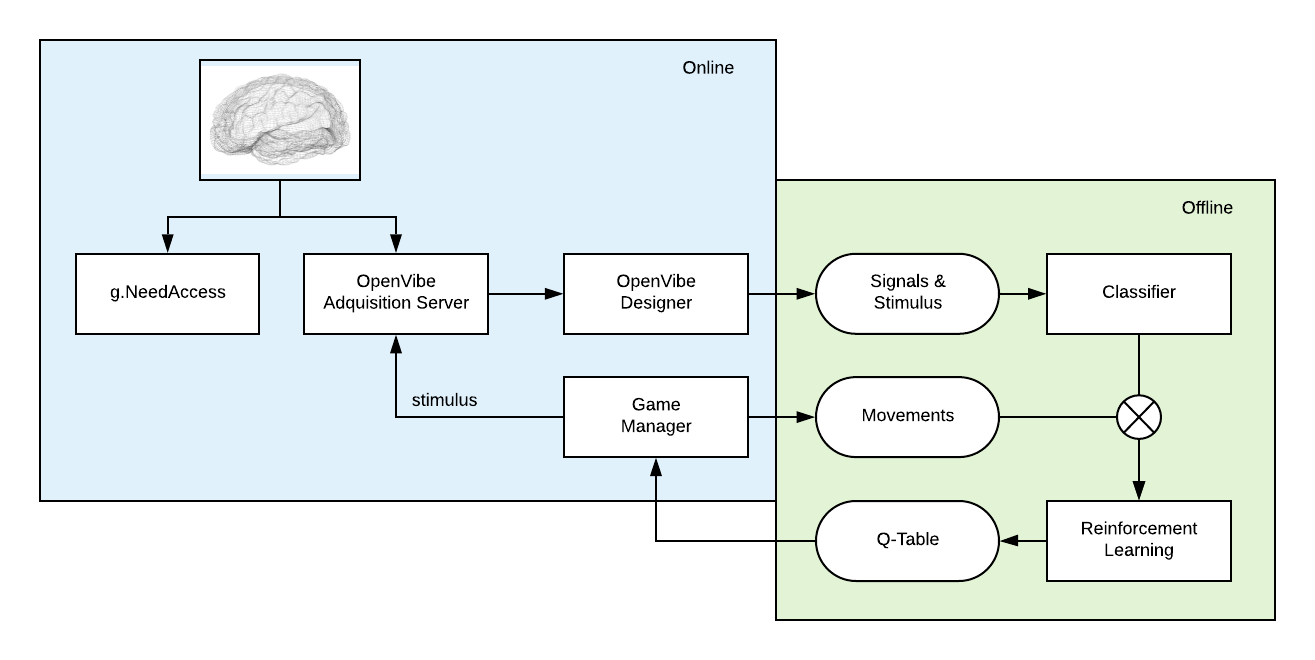
\includegraphics[scale=0.4]{Images/complete_flow.png}
    \caption{Overview of the experimental procedure.}
    \label{diag:complete_flow}
\end{figure}

The experimental procedure is summarized in Figure \ref{diag:complete_flow}. The core of the procedure is the retrieval of the subject's brain activity. This process is called brainwave session. In order to fetch this data, subjects use a wireless digital EEG device during the experiment (g.Mobilab, g.Tec, Austria). Once the subject has the headset on, a set up procedure is executed to implement an impedance check and to visually inspect the EEG signals in order to verify if it the electrophisiological interface is generating valid data. Subsequently, the OpenVibe Acquisition Server, from the OpenVibe platform~\cite{OPEN-VIBE-PAPER}, is launched and configured. This program has the responsibility of receiving the signal data from the headset and any event information from the game and transfers it to the OpenVibe Designer application. After this step, the Game and the OpenVibe Designer programs are launched and configured to communicate with the previously mentioned acquisition server. Once the subject is ready, a computer screen is positioned in front of her and the brainwave session starts. A brainwave session consists of several experiences, each one being a game run, and it uses a pseudo-random function to determine the agent's movements. The system is described in more detail in Section \ref{cognitive_experiment_system} and the brainwave session in Section \ref{cognitive_experiment_details}. Once the experimental procedure is completed, the game state information and the signal data with the game event information of each run are stored. For each run, the signals and stimulus information are then passed to the classification module that uses them to train the classifier. The classification step is covered in detail in Section \ref{signal_processing_and_classification}. After this step is finished, the game movements and the trained classifier are used to update a Q-Table for each experience. Lastly, the calculated Q-Table is used to test if the agent has boosted its performance while playing the game. This module is explained in Section \ref{q_learning_step}.

\subsection{Cognitive Game experiment}
\label{cognitive_experiment_details}
%This section details the game system characteristics, the brainwave session process and the retrieval and analysis of the generated data from the subjects interaction with the system.

\label{cognitive_experiment_system}{
The game parsimoniously consists of a $5x5$ grid of grey circular spots with a black background.  A blue spot indicates current position of the agent whereas a a green spot represents the goal, as shown in figure  \ref{fig:game_representation}. The objective of the system is for the agent to reach the goal. The circular spot representing the goal remains static at the bottom-right position of the grid, while the one representing the position of the agent always starts at the upper-left position of the grid.  When the agent reaches the goal, the position where the agent and the goal are located turns red, showing that the experience has ended. There are four possible movements that the agent can perform: it can go upwards, downwards, towards the left and towards the right, and those moves are bounded to avoid the agent from leaving the grid. The movement direction is selected randomly and is executed once every 2 seconds.  When the experience ends, there is a pause of 5 seconds before the next experience starts. Each time an agent moves, it is considered as a stimulus to the observational human critic.  The experience is designed for it to be evident whenever there is an error (i.e. the agent moves away from the objective) so the subject can notice it immediately after the stimulus is presented, possibly triggering the expected cognitive response, which can be imprinted as an ErrP component within the EEG stream.

\begin{figure}[h!]
\begin{subfigure}{0.5\textwidth}
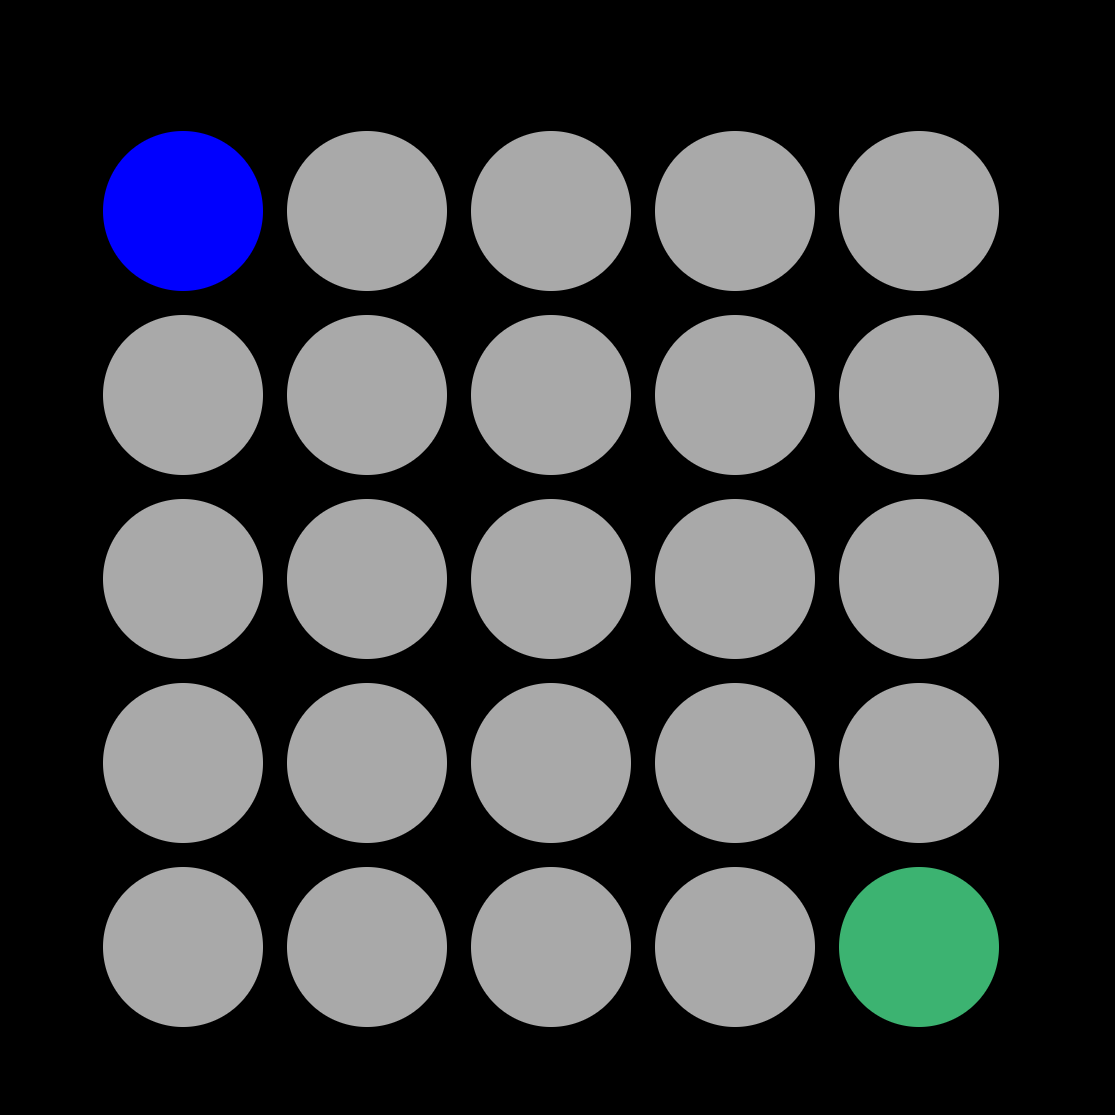
\includegraphics[width=0.9\linewidth,scale=0.9]{Images/grid_initial_state.png} 
\caption{Initial state of the grid.}
\label{fig:subim1}
\end{subfigure}
\begin{subfigure}{0.5\textwidth}
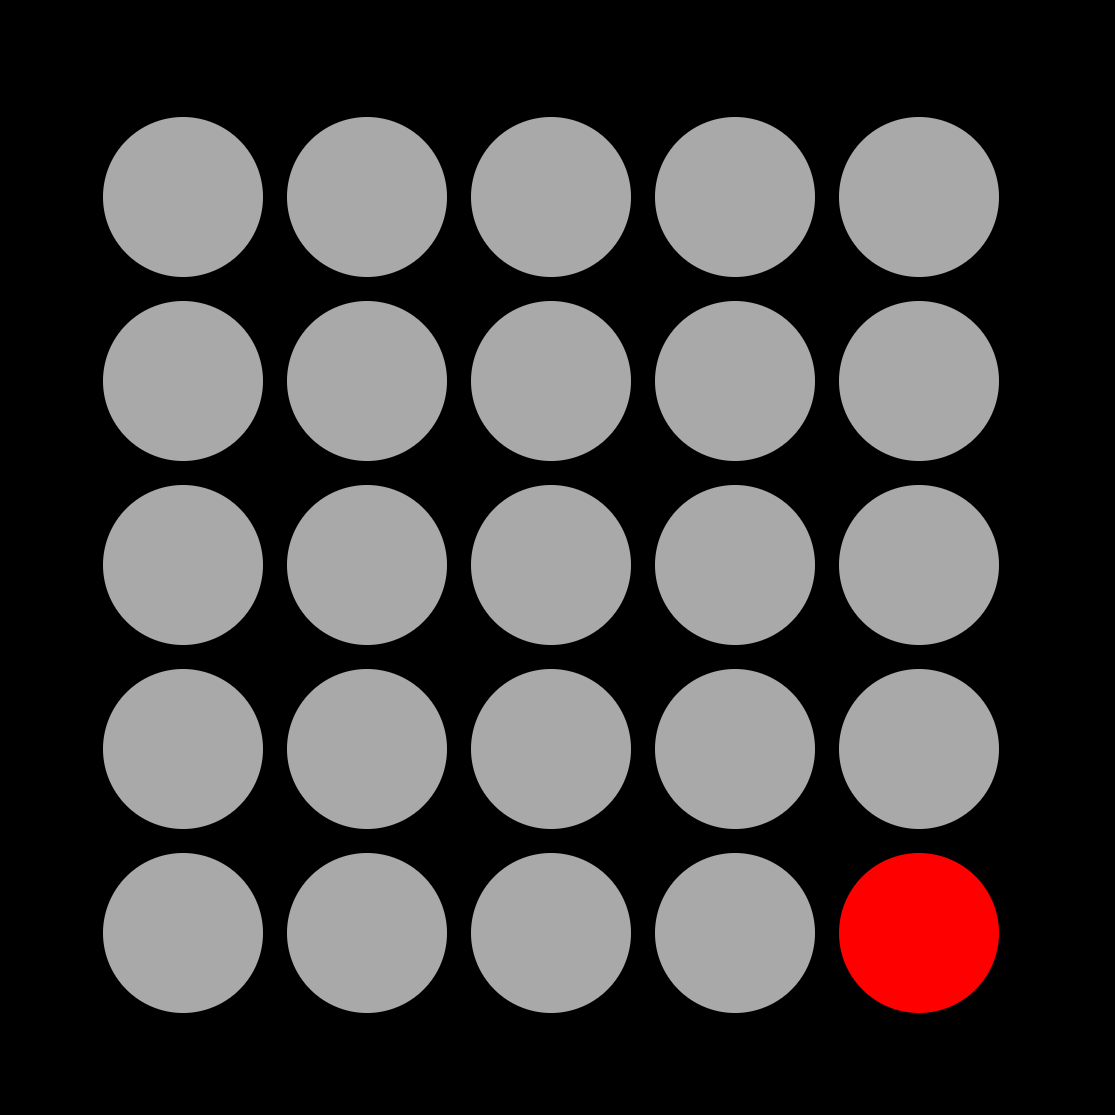
\includegraphics[width=0.9\linewidth,scale=0.9]{Images/grid_end_state.png}
\caption{Final state of the grid.}
\label{fig:subim2}
\end{subfigure}
\caption{Grid system representation used in cognitive experience.}
\label{fig:game_representation}
\end{figure}
}

\section{Calibration}
\label{section:calibration}

The first step in order to be able to find ErrP signals is to choose the most efficient algorithm, and the proper calibration. In order to do this different parameters are tested for a set of algorithms and for each individual subject. Initially a sub-selection of experiments is used to define a subset of parameters to test with, and then all the data is tested with this subset of parameters.

\section{Signal Processing and Segmentation}

To aid in detecting the ErrP response, an offline processing pipeline and classifier is constructed to identify whether the action taken by the agent is an error or not. It is developed in Python using the \href{https://mne-tools.github.io/0.11/index.html}{MNE} platform \cite{MNE-PYTHON}, which is a package designed specifically for processing EEG and MEG data, and the machine learning library \href{https://scikit-learn.org/stable/}{Scikit-Learn}.

Many classification methods are considered. The best classifier is selected based on a calibration and selection procedure that is further explained in sections \ref{algorithm_calibration} and \ref{algorithm_comparison}. After an optimal algorithm and a configuration are selected, a classifier is trained for each subject and then epochs from their experiences are classified. These classifications are then used by a reinforcement learning algorithm to train the agent. This last algorithm is explained in detail in section \ref{q_learning_step}.

This step consists of processing the collected signals in order to train a classifier that can decide whether an error potential is triggered or not. Firstly, the output of a brainwave session is read and a band pass filter of 0.1-20.0Hz is applied to the signal, as seen in Figure \ref{fig_psd_band_pass}. Samples that correspond to the start of an event are tagged using the data from the stimuli channel.

After the data is loaded and tagged, epochs are extracted from the raw data. Epochs consist of all the sample points that take place between the start of the event and 2 seconds later (time for each action to take place), resulting in 500 samples per channel, as the sample frequency is 250 Hz.

Samples that do not correspond to an epoch are not used. Also, epochs referring to the start or finish of the experience are excluded. This is done because the start and the end of the experience doesn't involve the agent taking an action, thus giving signals that should not be considered in the classification process.

In this way, the raw data of an entire brainwave session is processed into an array of experiences where each element is an array of epochs tagged with a number specifying if the epoch corresponds to an action that made the agent move further from the goal (hit) or an action that made the agent move closer to the goal (no hit). The ErrP is expected to be found in hits. To get the data ready for classification, the stimuli channel is removed in order to classify the signals using only the EEG data and a mne.decoding.vectorizer \footnote{Link to vectorizer documentation: \href{https://mne.tools/dev/generated/mne.decoding.Vectorizer.html}{https://mne.tools/dev/generated/mne.decoding.Vectorizer.html}} function is applied to transform the data into a single array sample. Lastly, this data is used by the classification module as information to train and test a classifier.

\section{Classification with Logistic Regression}
For the logistic regression algorithm the parameters that are tested are $C$ and the Solver.  The $C$ parameter is the inverse of the regularization strength. The values this parameter can take are 0.001, 0.01, 0.1, 1 and 10. The solver parameter refers to the algorithm that is used in the optimization problem, the ones that are tested are $lbfgs$ and $saga$. The different configurations that resulted as optimal for subjects can be seen in the apendix section \ref{apendix:algorithm_config:lr}.

Raw signals are classified using a vectorizer a minmaxscaler and finally the logistic regression classifier.  Even tough the classification accuracy is low, the information is enough to have valid rewards that can be used to retrieve the information.

\begin{figure}[h]
    \centering
    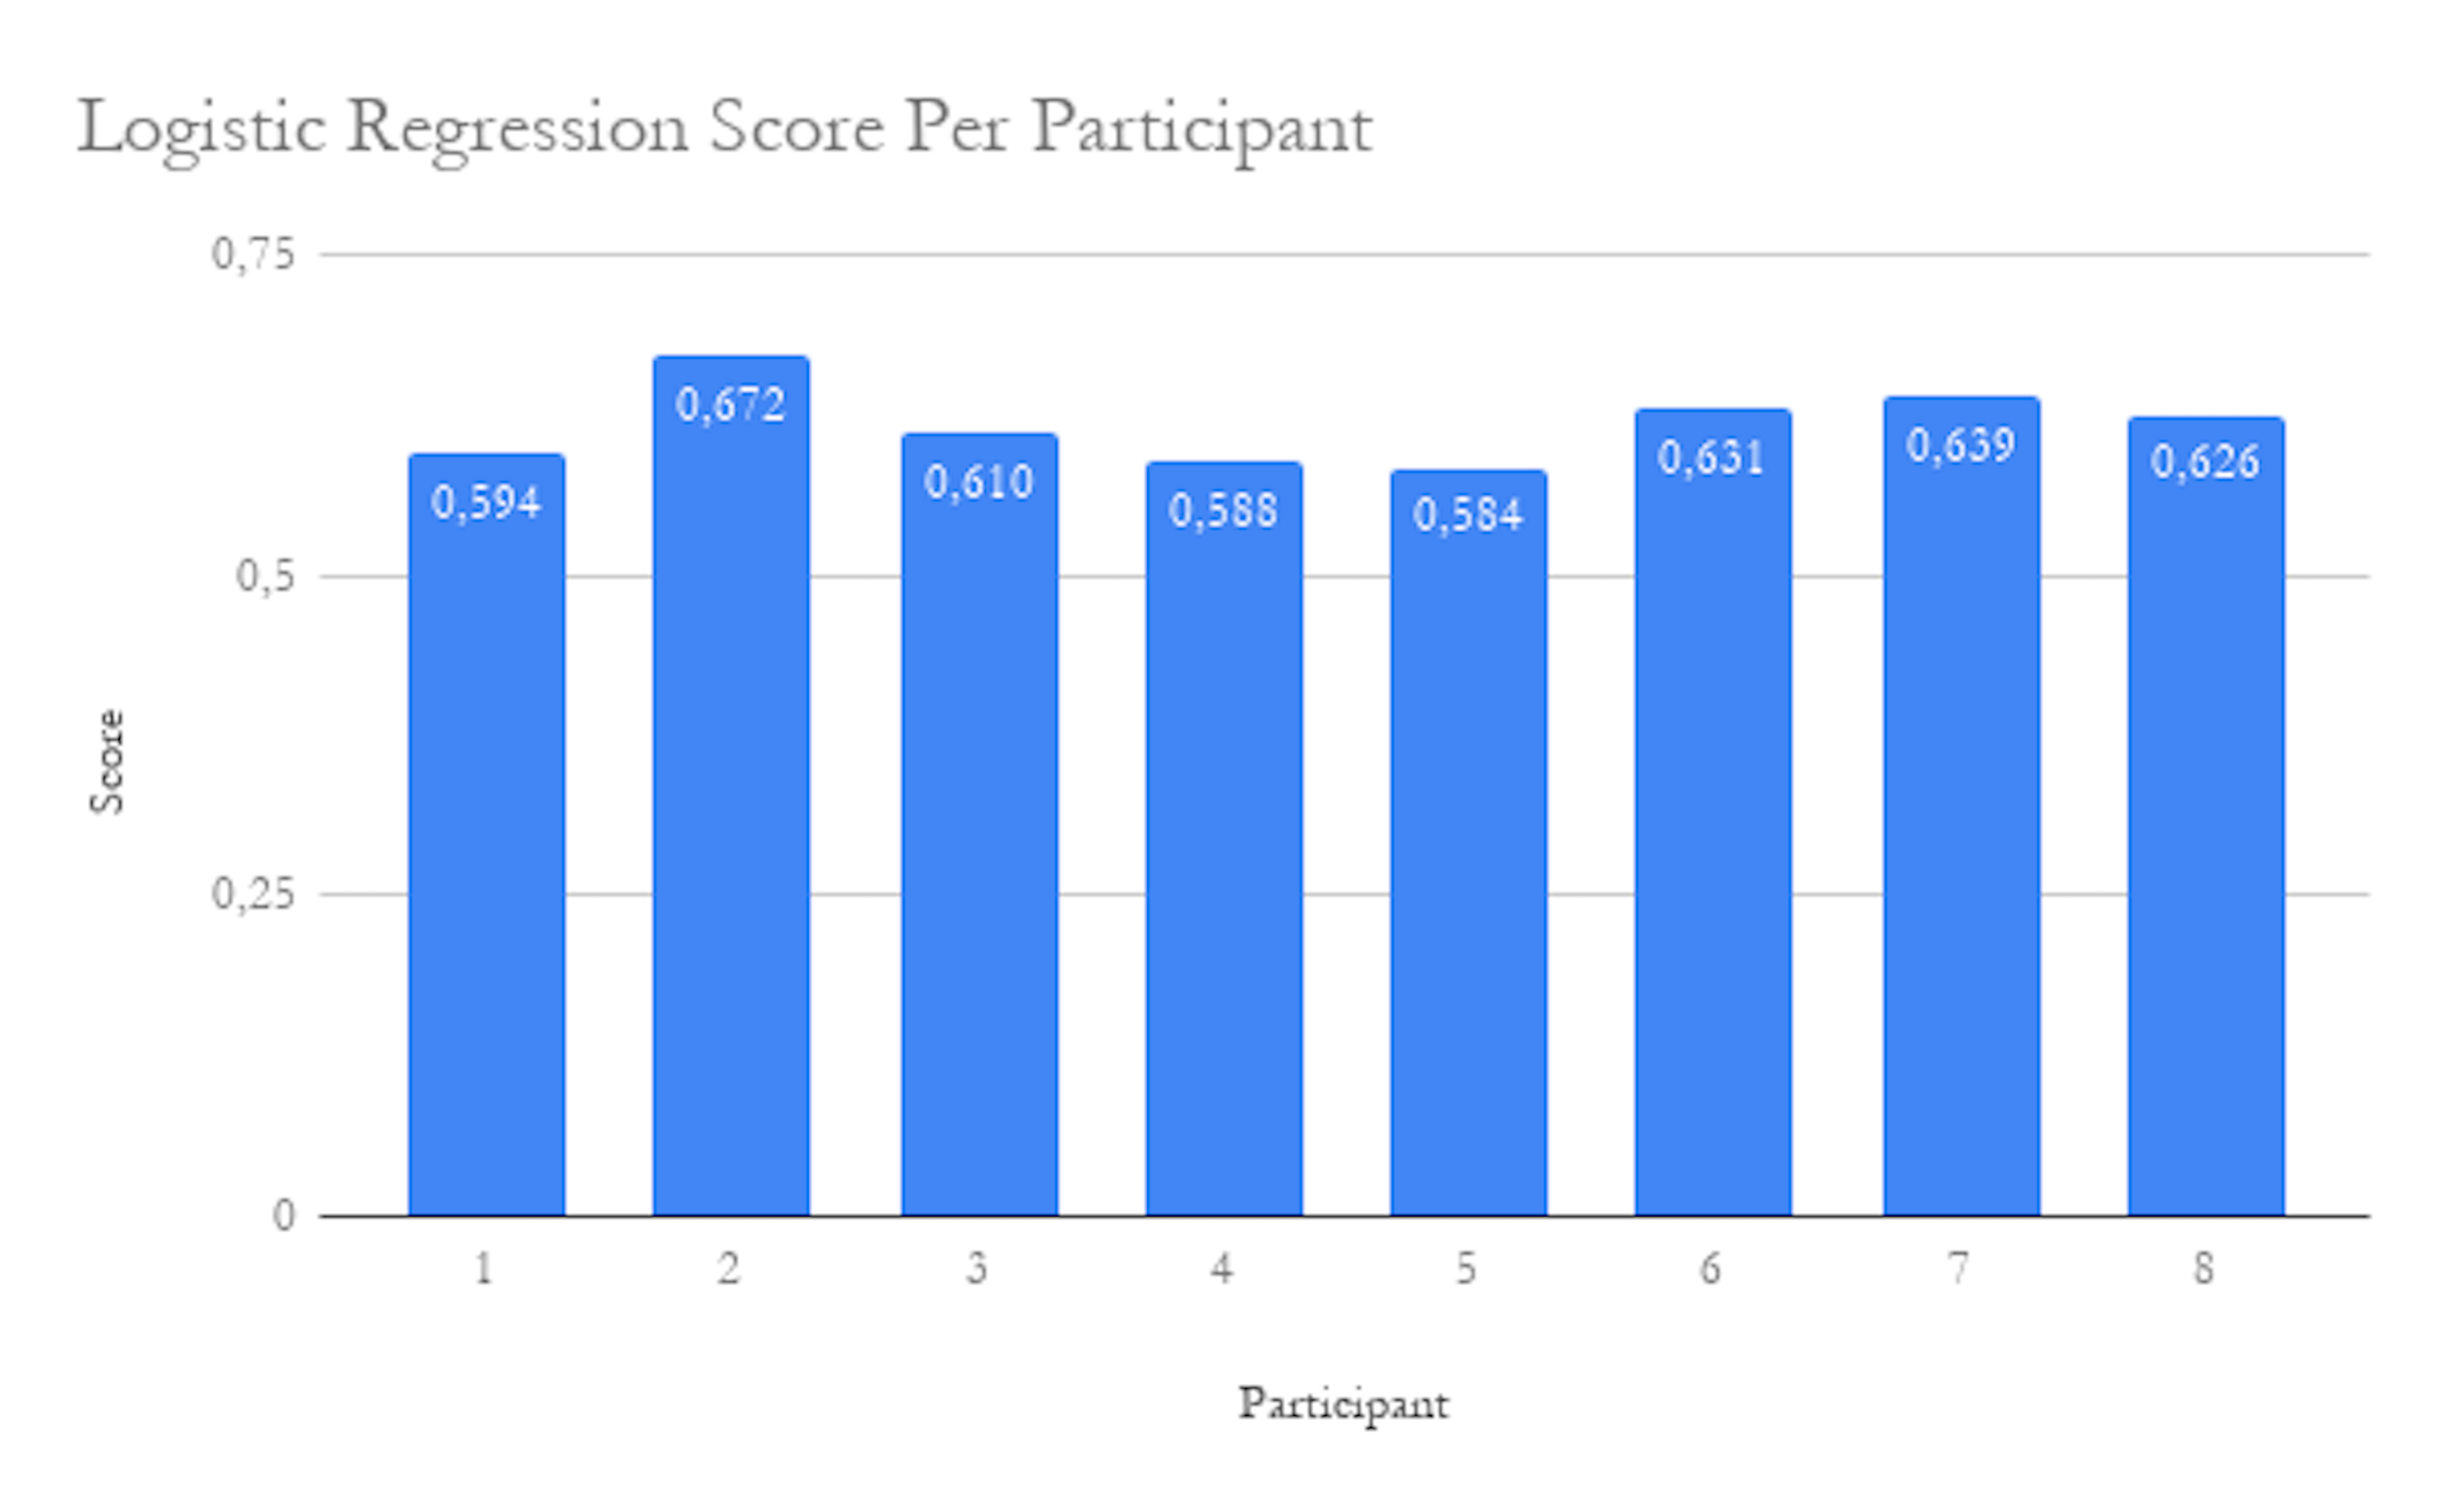
\includegraphics[scale=0.4]{Images/algorithm_calibration/LR_calib.png}
    \caption{Logistic Regression Algorithm Calibration}
    \label{diag:algorithm_calibration:lr}
\end{figure}

\section{Reinforcement Learning}

The set of experiences of each subject is split into training and testing, so that the results of the classification can then be used to improve the performance of the agent. After training the classifier, the testing experiences are classified. Then, for each experience a reward file is generated. For this purpose, game states files, which are submitted by the game when an experience takes place, are used. These files contain an ordered list of the states of the game throughout an experience. With this file and the classification of the test data of an experience, a reward file is submitted. This file specifies a reward for each movement in the game, based on the classification of the event that corresponds to that movement. The reward can either be -1 when the event is classified as a hit or 0 when it is classified as a no hit. The accuracy of this rewards depends on the performance of the classifier. This reward file is used by the Q-Learning algorithm to improve its performance, as detailed in section \ref{q_learning_step}.


\subsection{Q-Learning}{
\label{q_learning_step}
A Q-Learning algorithm is used to train the agent. It is developed in Python and uses the \href{https://gym.openai.com}{OpenAI Gym} toolkit. Gym is a toolkit for developing and comparing reinforcement learning algorithms. It makes no assumptions about the structure of an agent, and is compatible with any numerical computation library, such as TensorFlow or Theano.

\subsubsection{Algorithm implementation}{
\label{q_learning_step_alg}
The Q-Table is initialized with zeros, unless a preexisting Q-Table is passed as a parameter. In order for the agent to learn from the feedback generated by the subject, the Q-Table is not used to determine the action to take at a given state. Instead, the policy which determines which action to take in a particular state is given by the steps taken from the brainwave session results. This allows to train the Q-Table based on the subject's feedback from the movements the agent took, which are chosen pseudo-randomly, while executing the brainwave session. The previously mentioned feedback is not explicit as it comes from the interpreted brain signal data, which is collected while the agent is executing the brainwave session and then each action is classified as an error or not. This implies that the reward is determined by the subject's brain activity. This is covered in further detail in \ref{q_learning_step_env}.

While using the previously mentioned step function, the Q-Table is updated in each iteration. This is done following the Equation \ref{equ:update_q_table}.

\begin{equation}
    Q(s,a) \leftarrow Q(s,a) + \alpha[r+\gamma* Max(s, a)-Q(s, a) ]
    \label{equ:update_q_table}
\end{equation}

After the algorithm finishes iterating through all the training episodes, the Q-Table is saved. Each experience is one $trainingEpisode$.

The reward function is calculated based on the current distance to the goal, if it has increased compared to the previous step then the rewards is negative, if not it returns zero. In order to test how the Q-Table is trained when the accuracy is not perfect the reward function doesn't always return the correct reward. It calculates a random number between 0 and 1, and if it is larger than the accuracy then it will return 0 even if it should return -1 as the reward.

The reward function is described in algorithm \ref{algorithm:env_rewards}.

\begin{algorithm}
\SetAlgoLined
\DontPrintSemicolon
$reward \leftarrow 0$\\
  \uIf{currentDistanceToGoal > previousDistanceToGoal}{
    $reward \leftarrow -1$ \;
  }
  \uElseIf{random.uniform(0, 1) < accuracy}{
    return reward \;
  }
  \Else{
    return 0 \;
  }
\label{algorithm:env_rewards}
\caption{Reward Calculation for $ChaseEnv$}
\end{algorithm}
}
}



\section{Results}

Enfatizar la idea de que la mejor métrica de la propia detección está dada por la propia capacidad del agente de minimizar su tarea, que hay un flujo de información que involucra la propia percepción de la persona.

\subsection{Reinforcement Learning}

\textbf{Average steps to goal}
Figure \ref{fig:avg_steps} shows the average amount of steps it takes to reach the goal as the Q-Table is progressively trained using the reward information obtained for each subject. Each point corresponds to the average amount of steps it takes for the agent to reach the goal for a specific Q-Table in 200 iterations. The first point represents the amount of steps it takes to reach the goal for a Q-Table that hasn't been trained at all, where movements are decided randomly. The next point corresponds to the amount of steps it takes to reach the goal using a Q-Table trained with one experience, and so on.

The results show that as the Q-Table is progressively trained the average amount of steps decreases, meaning that the agent learns. However, the rate at which it learns varies per subject, certain subjects have more effective experiments than others, for example results for subject 1 (fig \ref{fig:avg_steps_1}) show faster learning than those of subject 8 (fig \ref{fig:avg_steps_8}).

In the case for subject 5 and 6, the reward information obtained from the brainwaves is not enough to train the agent effectively. Figures \ref{fig:avg_steps_5} and \ref{fig:avg_steps_6} show no apparent learning, as the amount of steps to reach the goal doesn't decrease when trained. Both subjects have less recorded data from the sessions in comparison to the rest of the subjects. In particular, subject 5 has less recorded experiences, so it is respective graphic shows the amount of steps for an empty Q-Table and for a Q-Table trained with only one experience. These results are consistent with fig. \ref{fig:roc:manuel} and fig. \ref{fig:roc:marta}, which show that the signal classification for these subjects hasn't been particularly successful. The average steps result for these subject are similar to that of fig. \ref{fig:roc:noise} which is constructed from noise, so the generated Q-Table would be similar to one generated with noise.


\begin{figure}[h!]
\begin{subfigure}{0.5\textwidth}
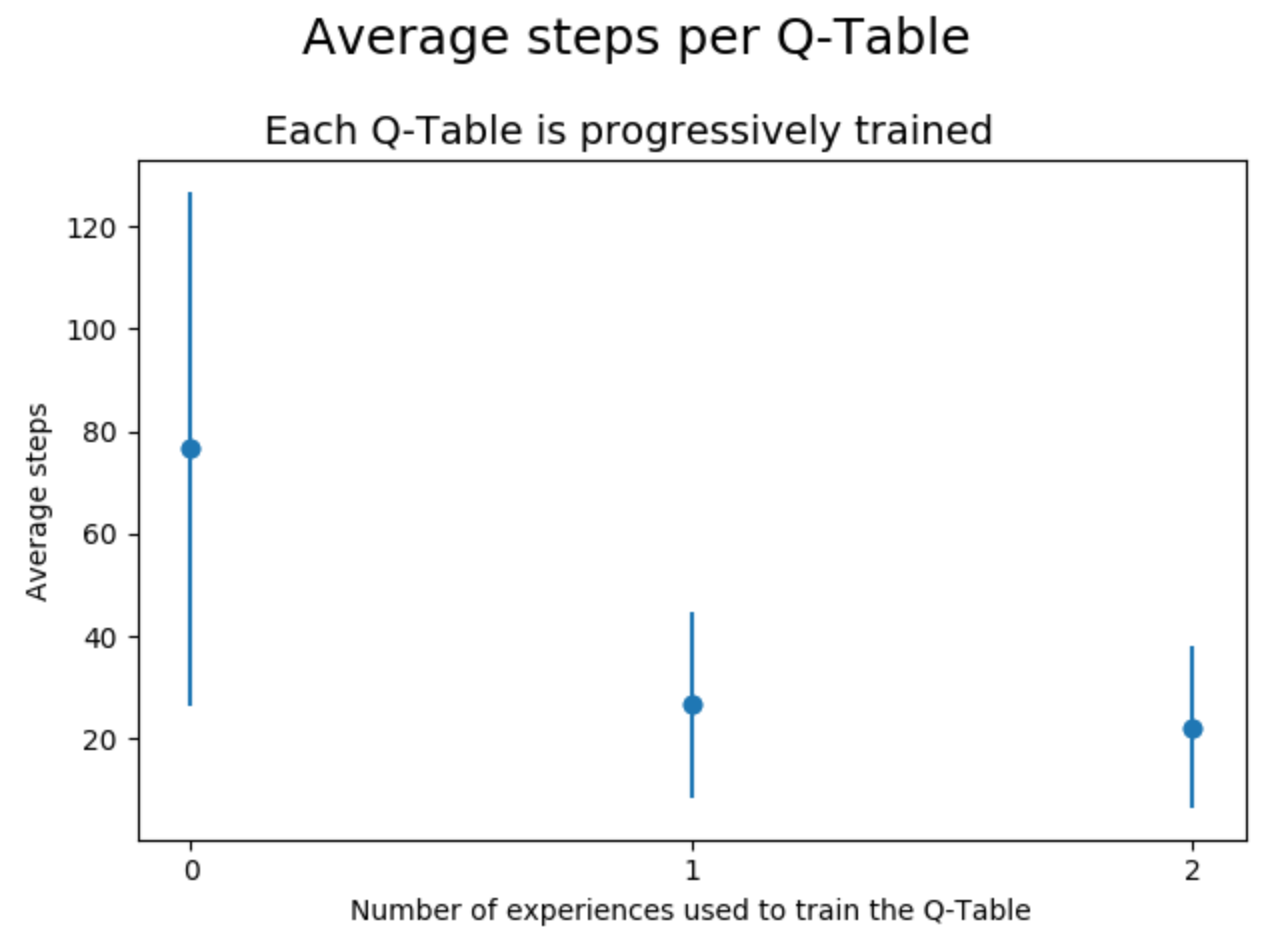
\includegraphics[scale=0.2]{Images/Average_steps/alex.png}
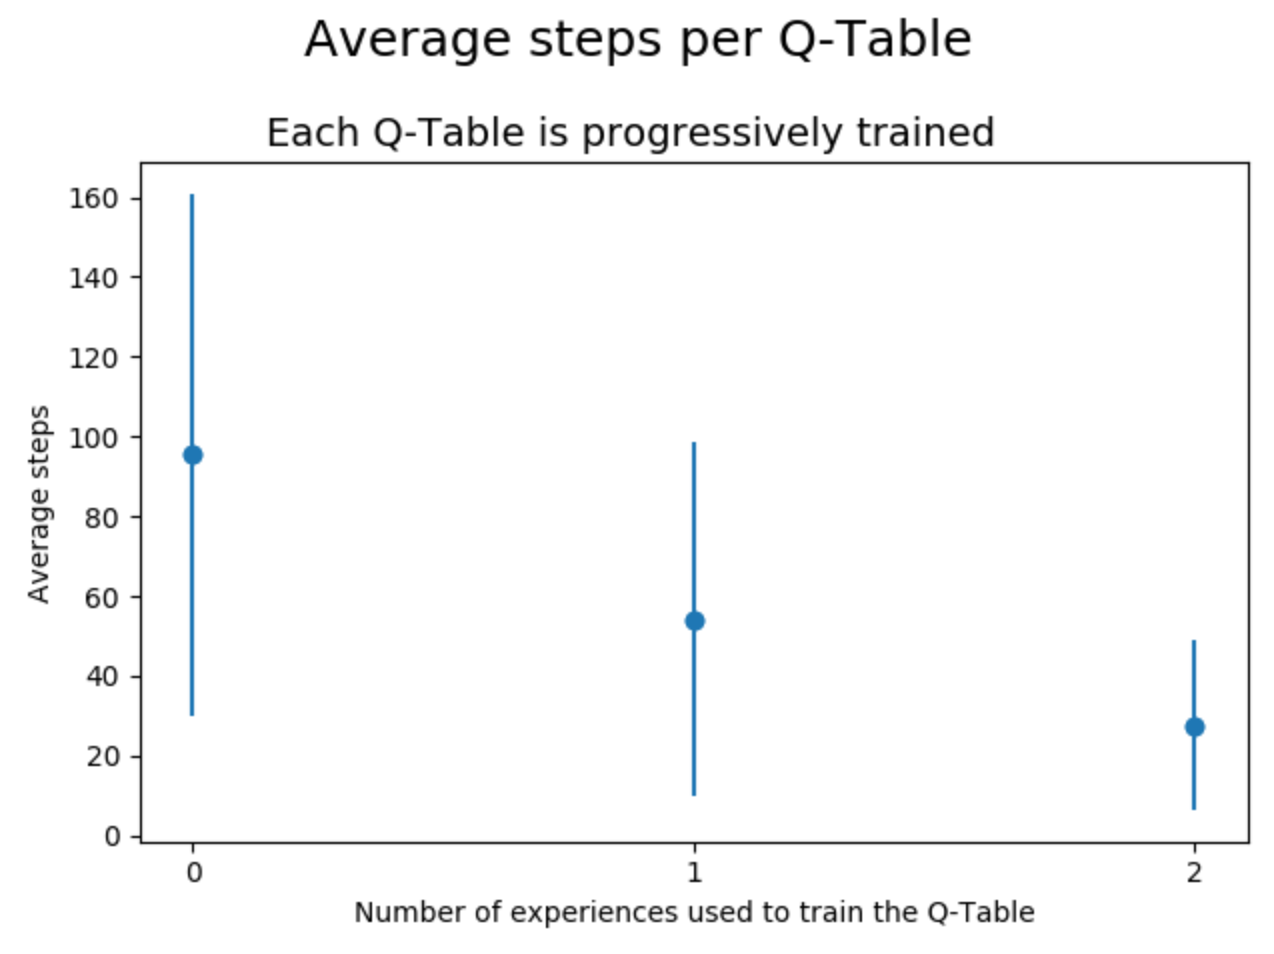
\includegraphics[scale=0.2]{Images/Average_steps/gonza.png}
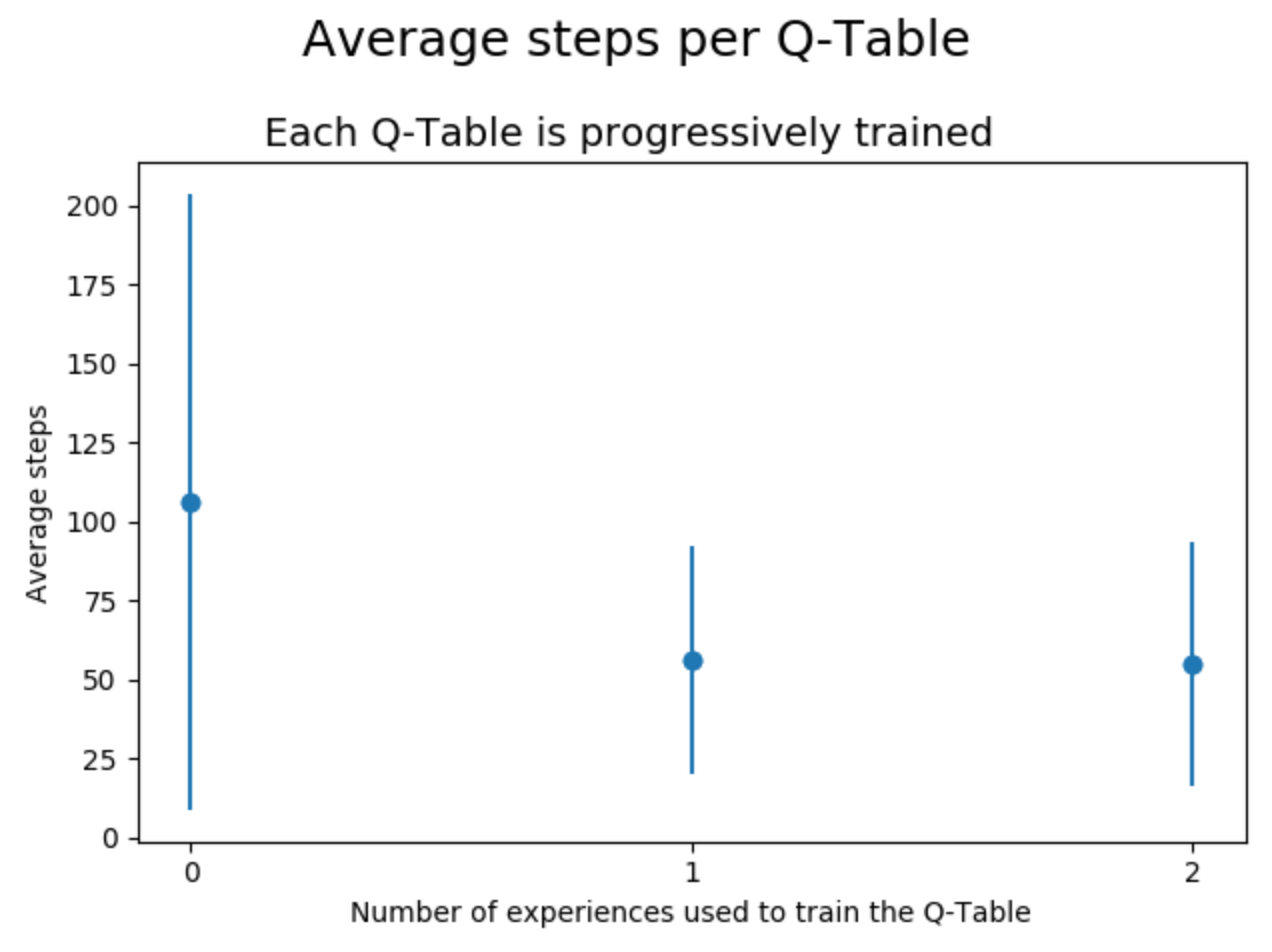
\includegraphics[scale=0.2]{Images/Average_steps/jose.png}
 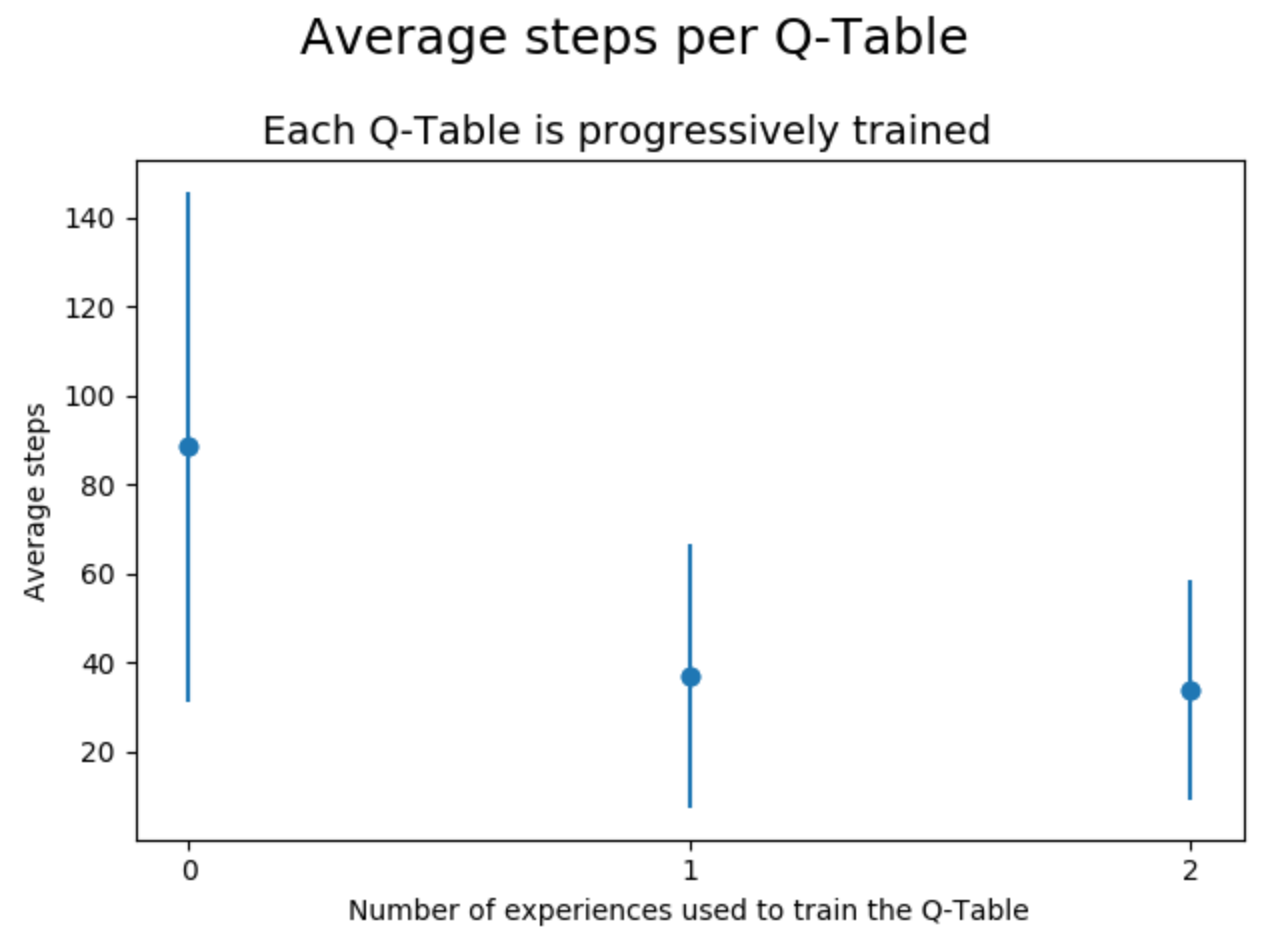
\includegraphics[scale=0.2]{Images/Average_steps/juan.png} 
\caption{Initial state of the grid.}
\label{fig:subim1}
\end{subfigure}
\begin{subfigure}{0.5\textwidth}
 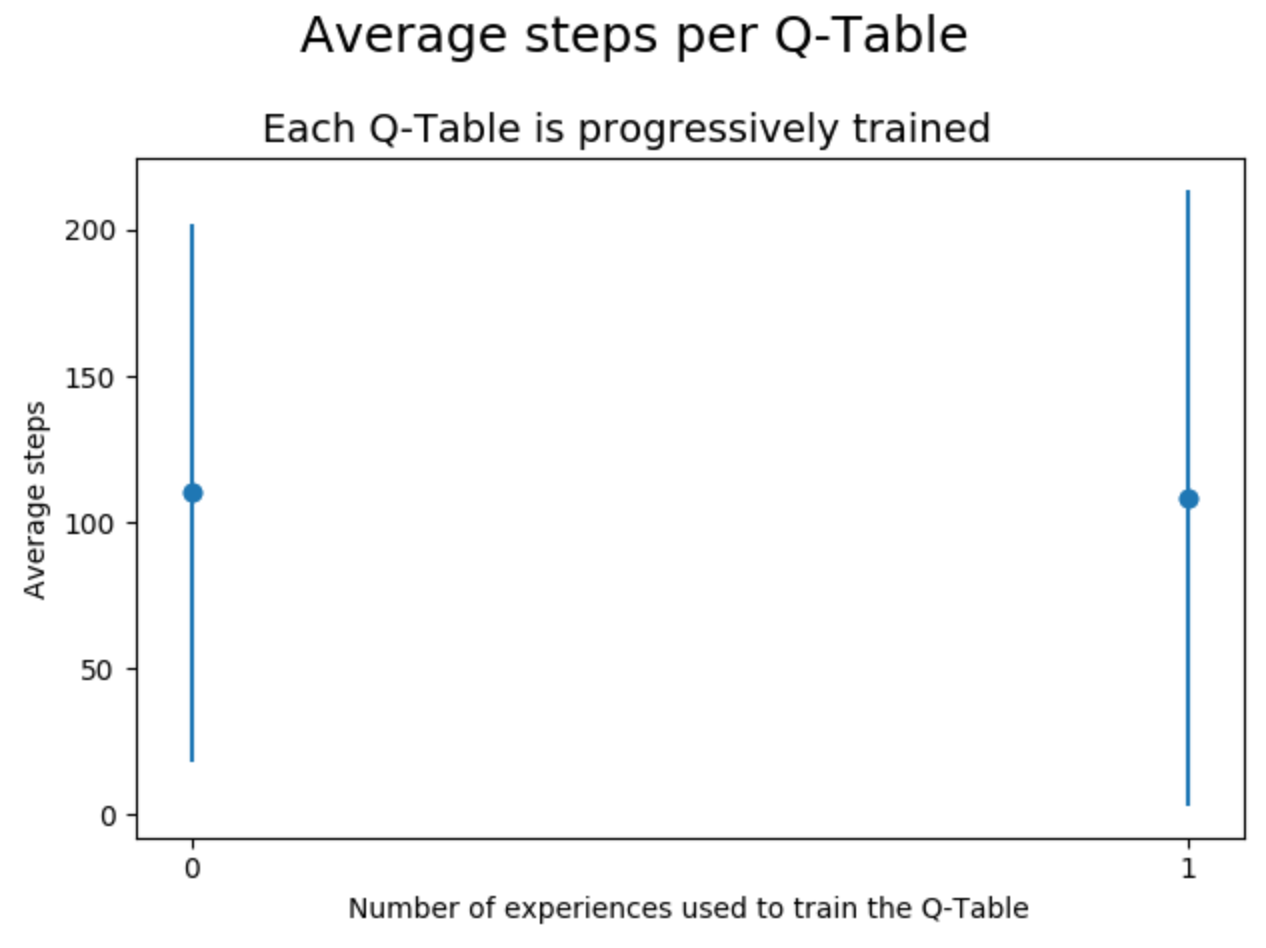
\includegraphics[scale=0.2]{Images/Average_steps/manu.png} 
  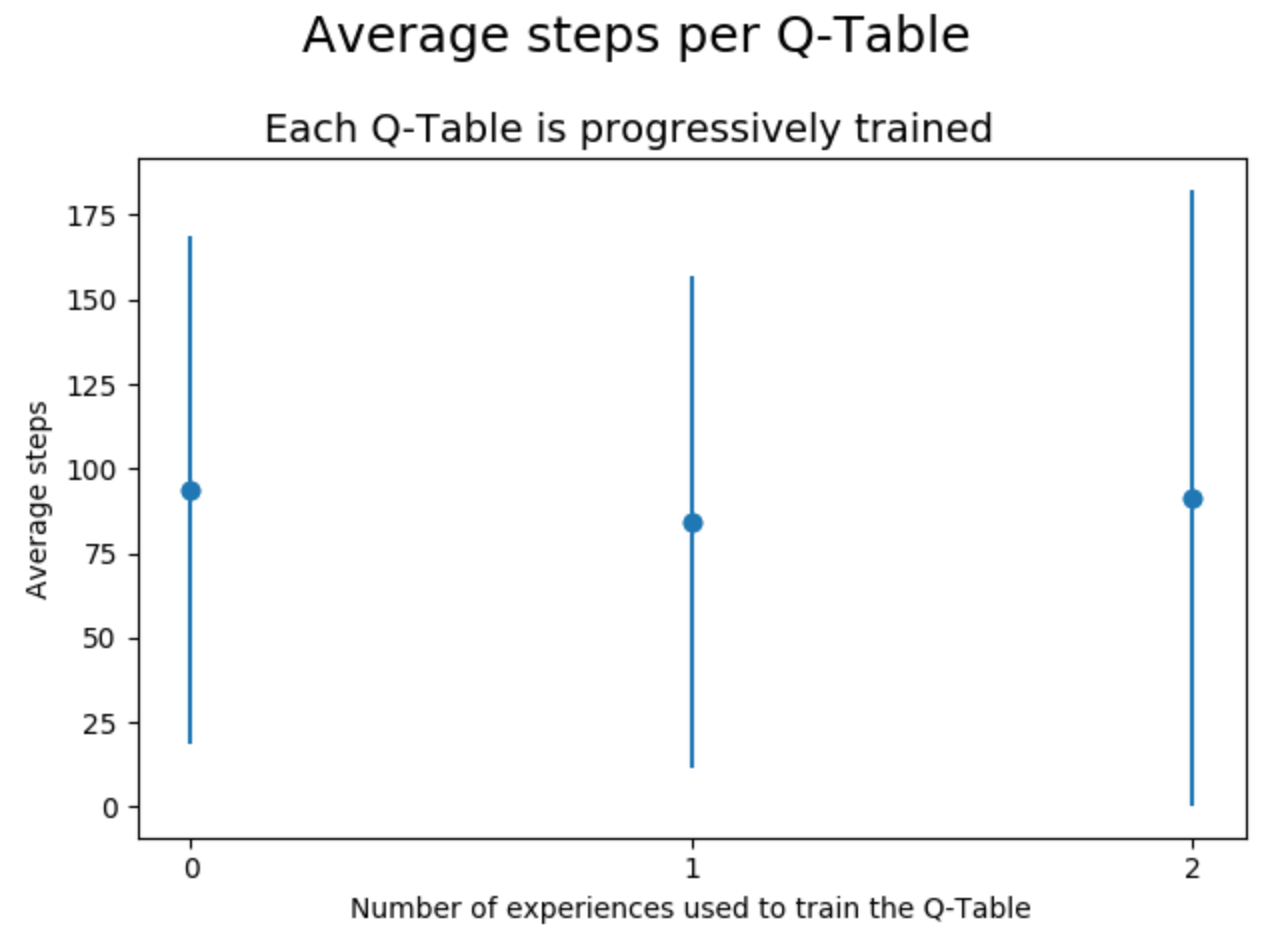
\includegraphics[scale=0.2]{Images/Average_steps/marta.png} 
  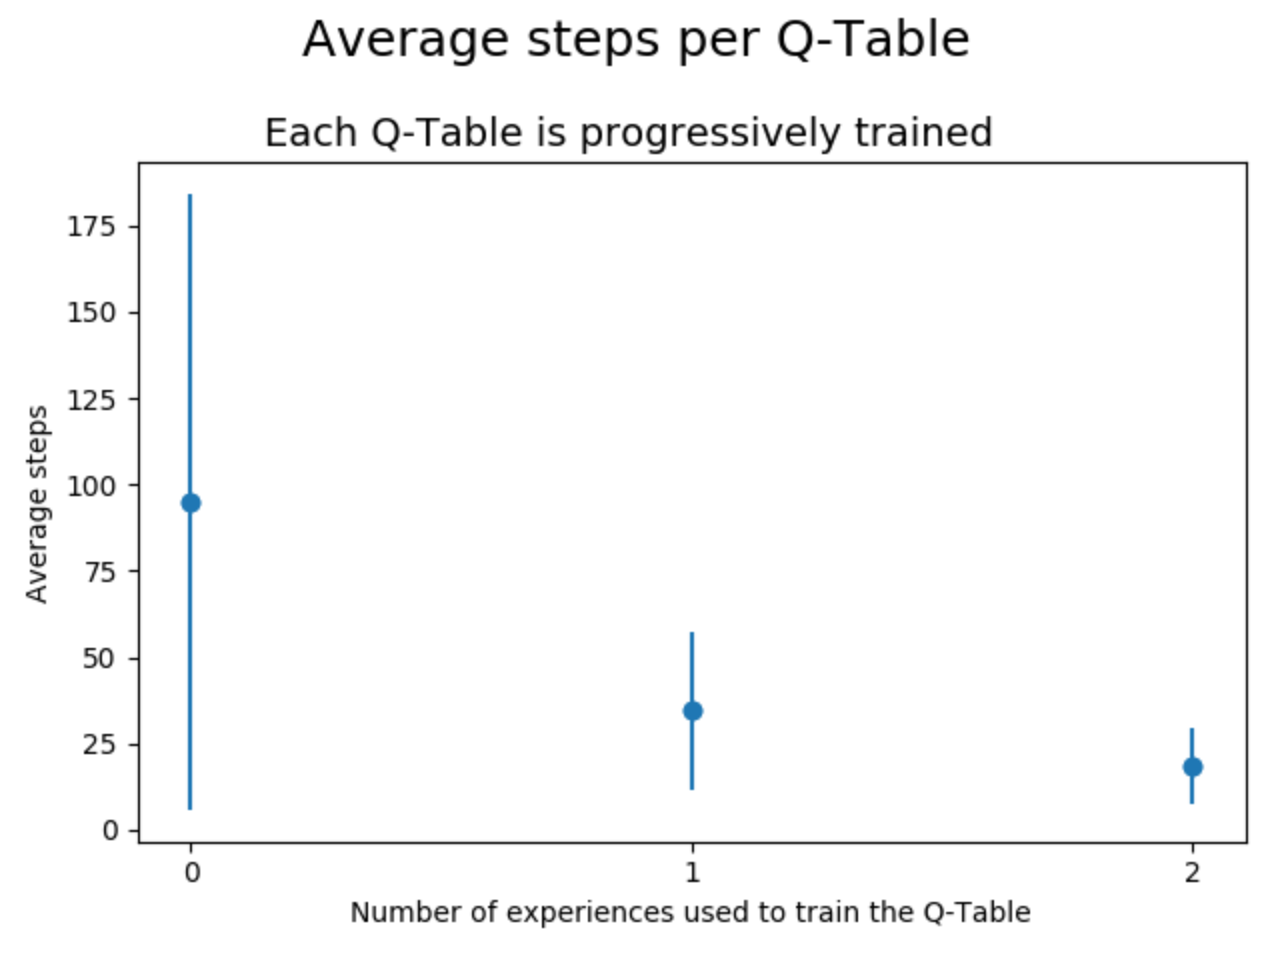
\includegraphics[scale=0.2]{Images/Average_steps/nati.png} 
  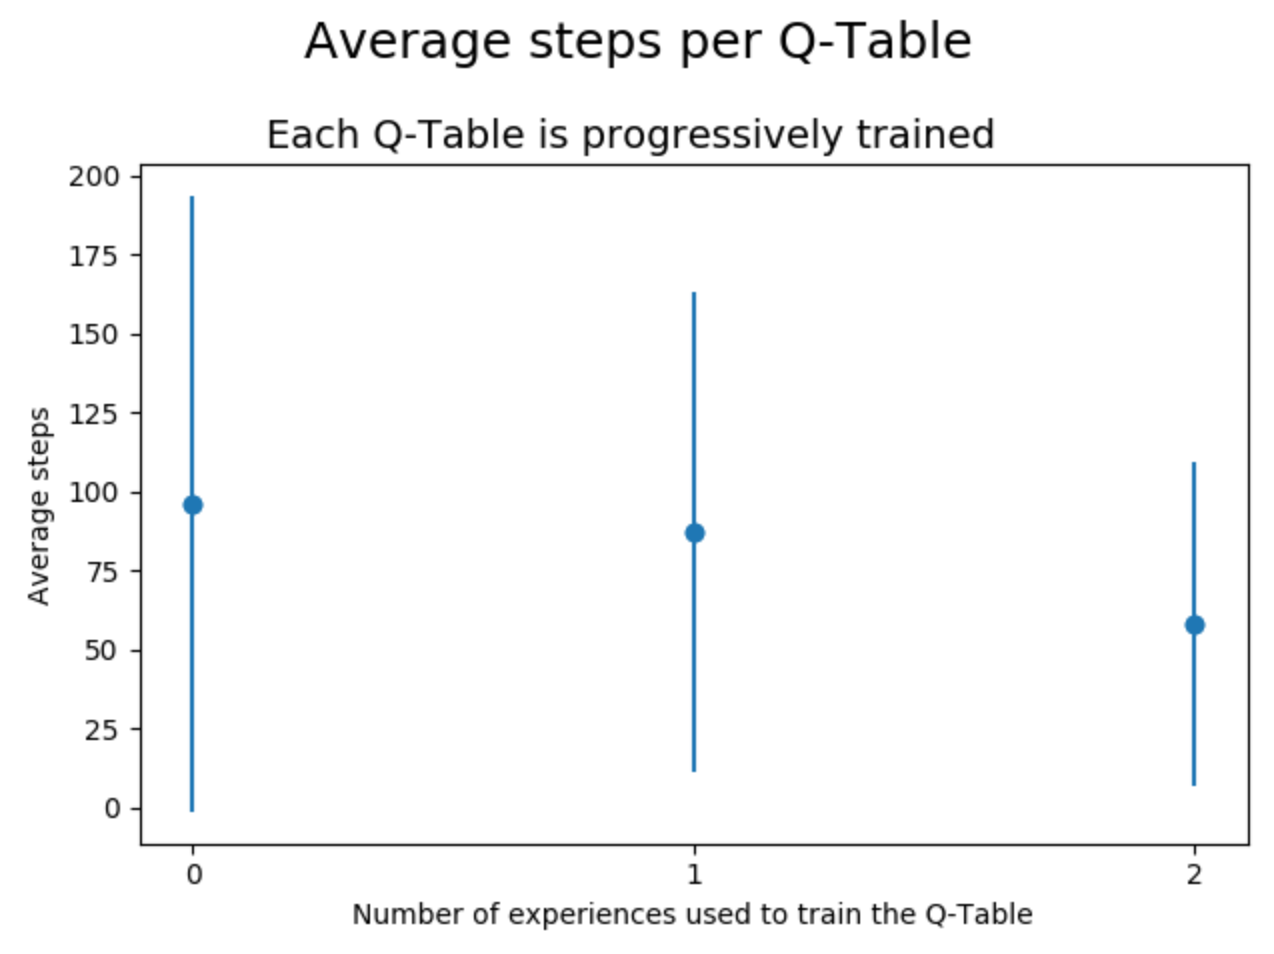
\includegraphics[scale=0.2]{Images/Average_steps/santiago.png} 
\caption{Final state of the grid.}
\label{fig:subim2}
\end{subfigure}
\caption{Grid system representation used in cognitive experience.}
\label{fig:game_representation}
\end{figure}


\begin{figure}[h!]
\centering
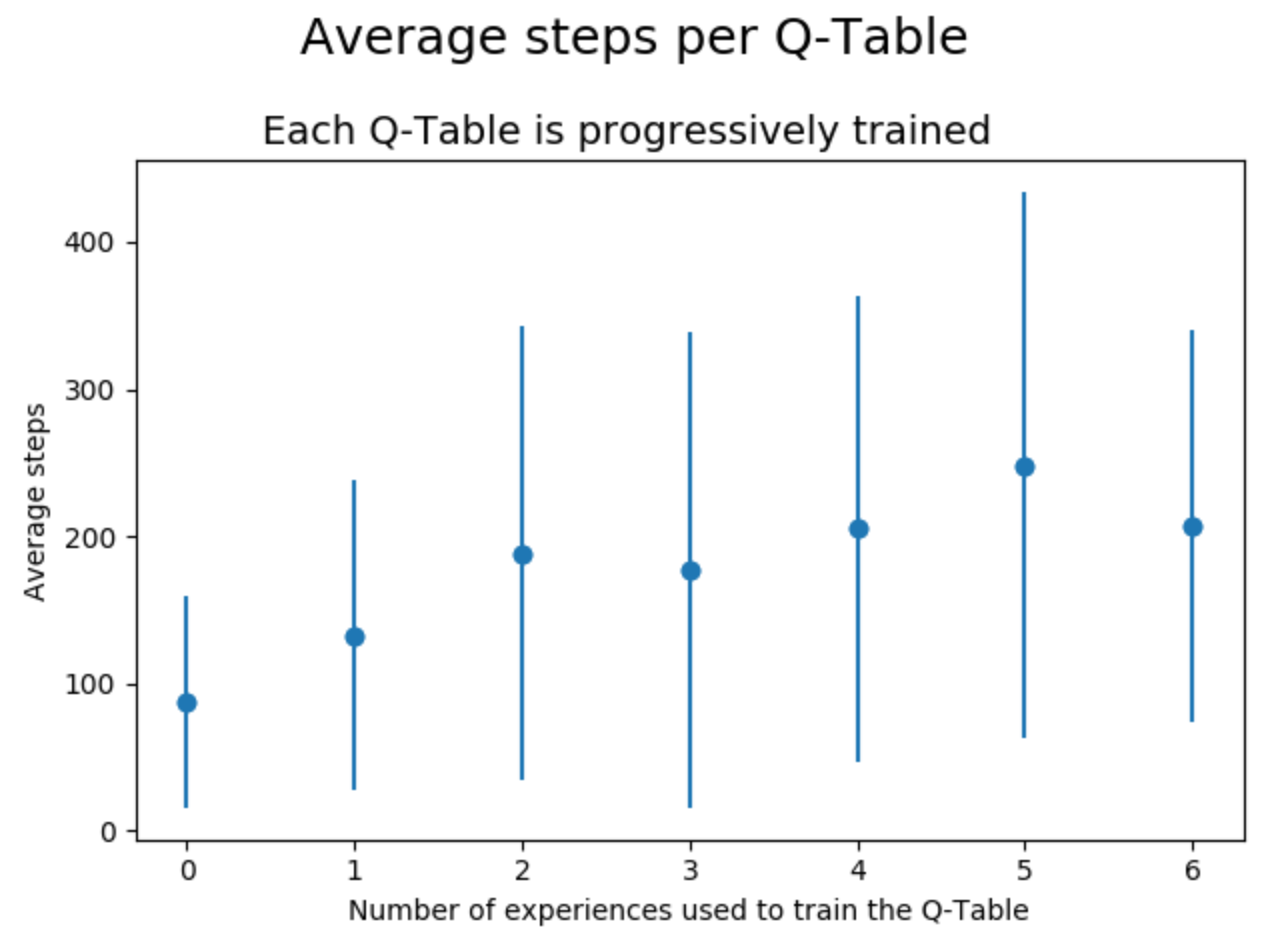
\includegraphics[scale=0.4]{Images/Average_steps/noise.png}
\caption{Average steps using Q-Table trained with noise.}
\label{fig:avg_steps_noise}
\end{figure}


\begin{figure}[h]
    \centering
    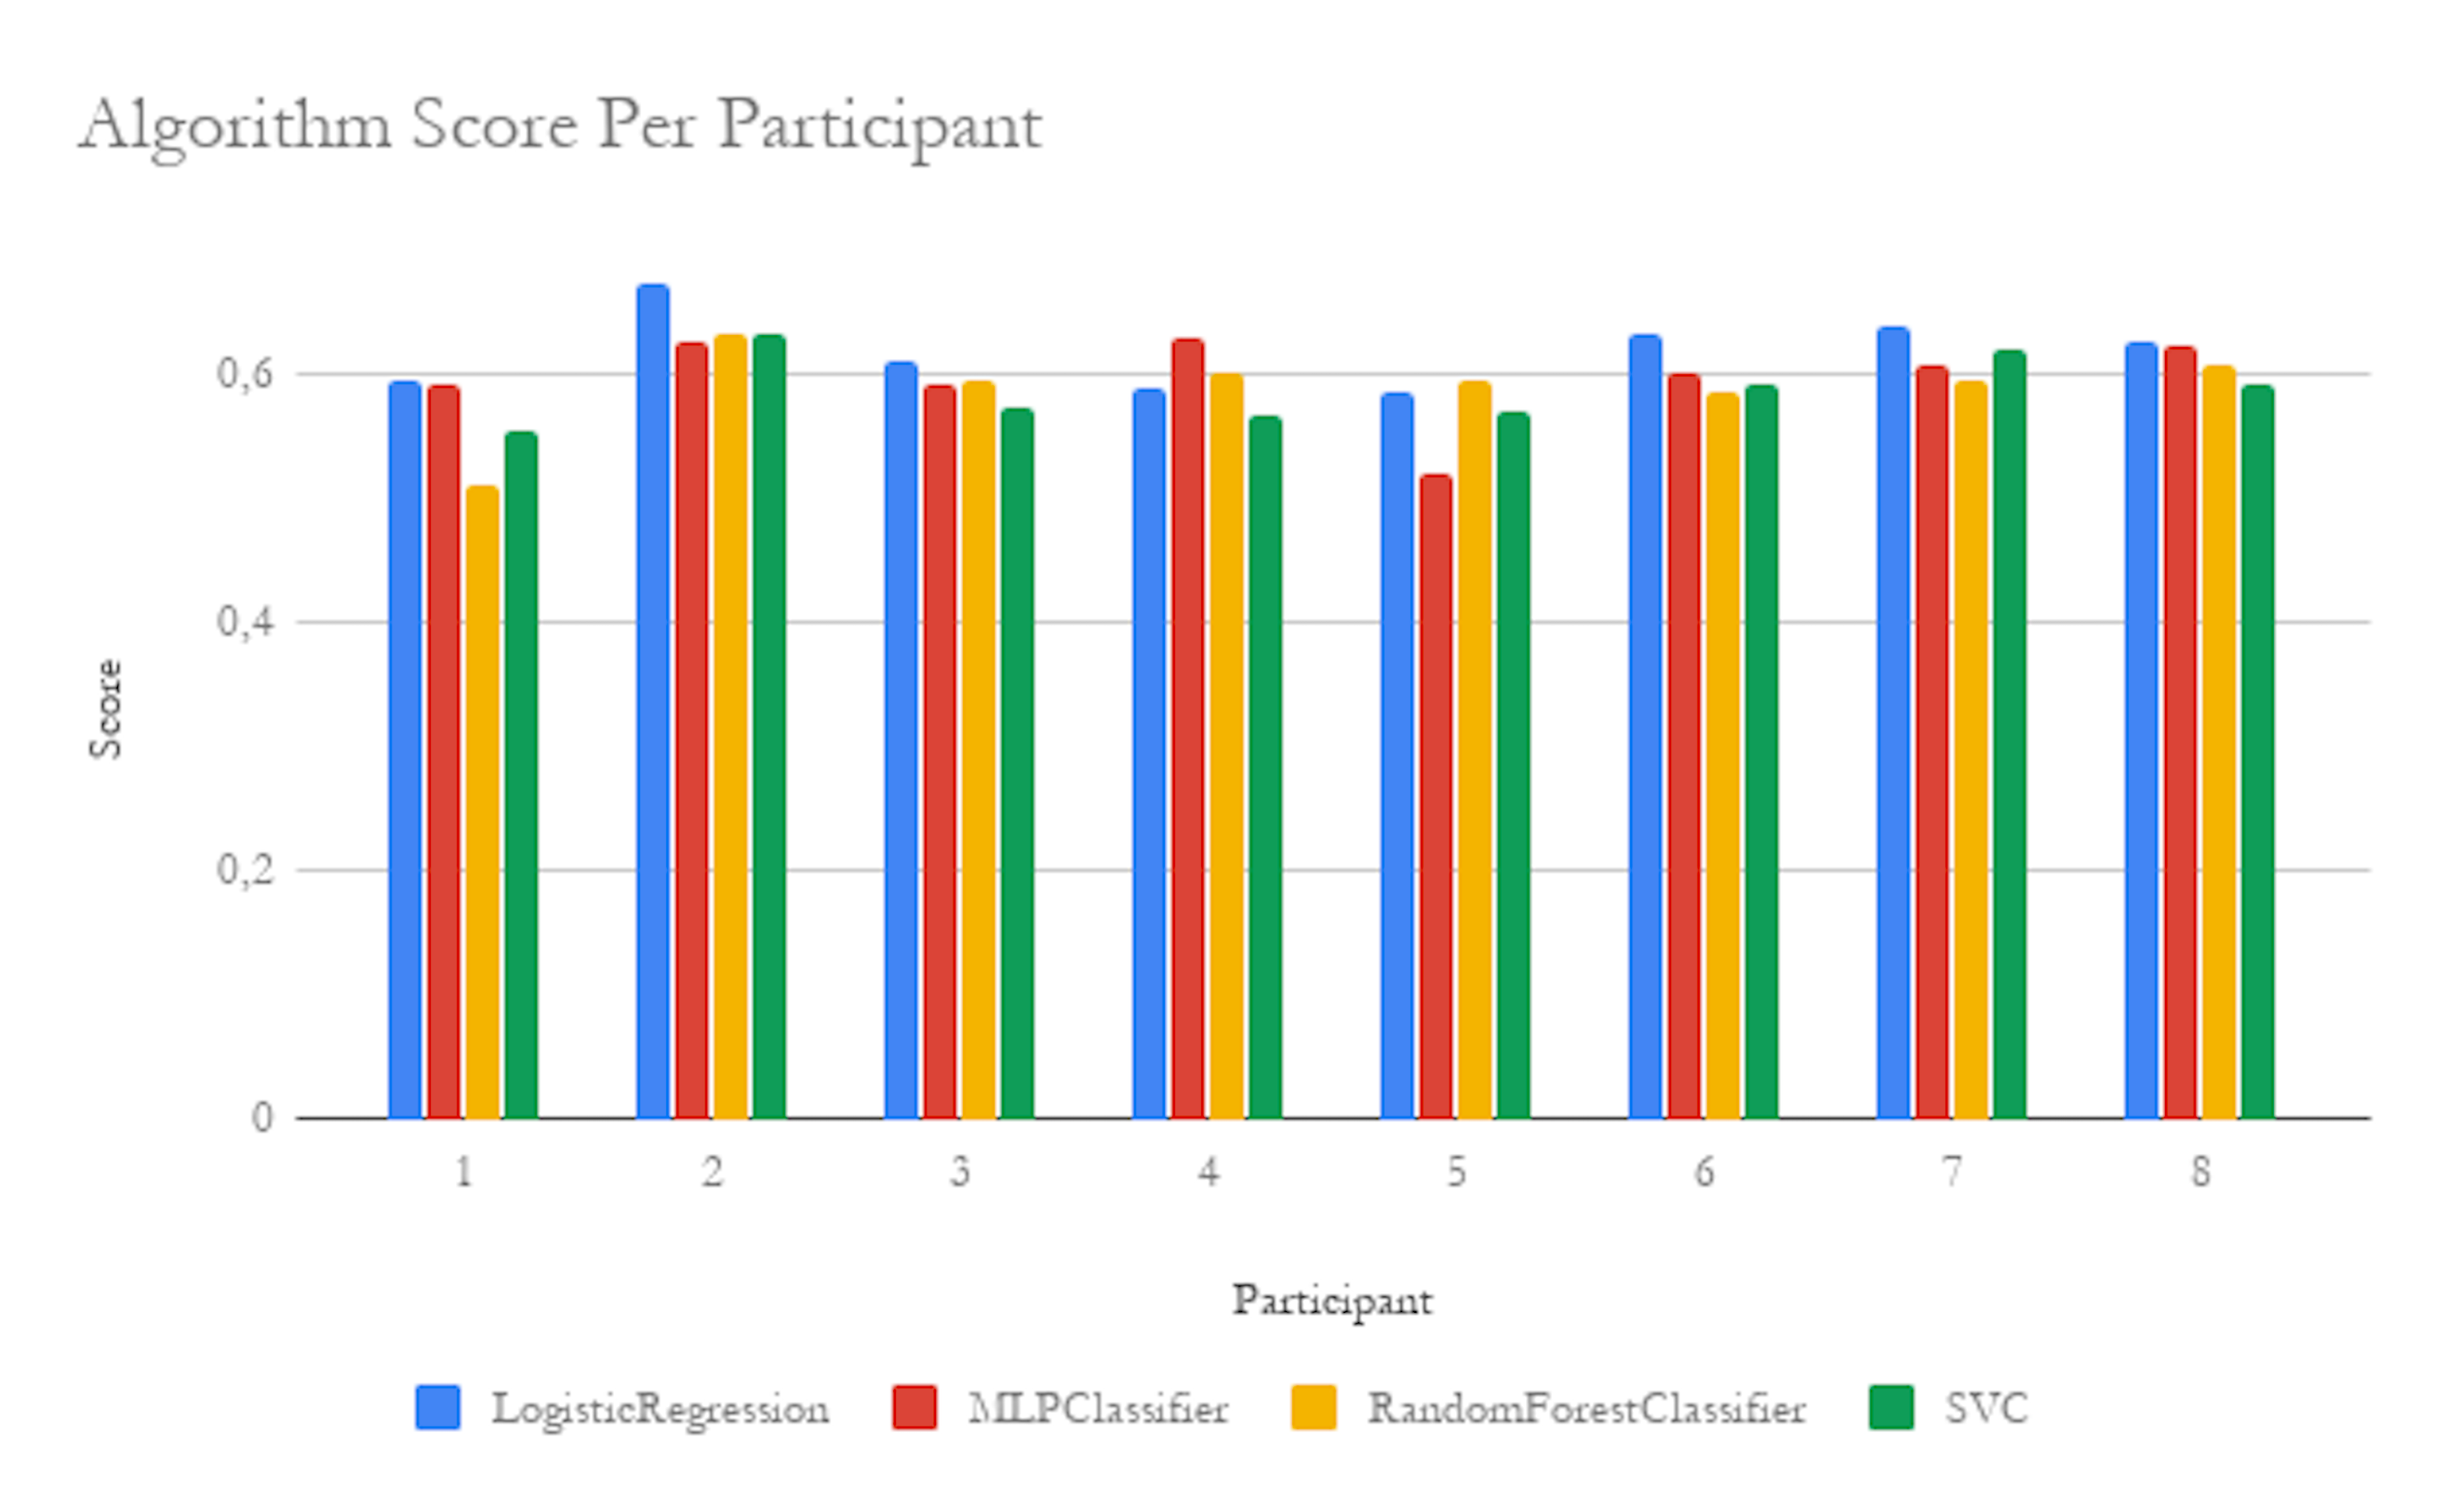
\includegraphics[scale=0.4]{Images/algorithm_calibration/Total_calib.png}
    \caption{Score Obtained With The Optimal Calibration Per Algorithm Per Subject}
    \label{diag:algorithm_calibration:subject_calib}
\end{figure}

\section{Conclusion}
The present research work set out to validate if ErrP signals could be used to train an agent using reinforcement learning. The collected data show that ErrP signals can in fact be classified and used to train an agent effectively. 

Enfatizar la idea de que la mejor métrica de la propia detección está dada por la propia capacidad del agente de minimizar su tarea, que hay un flujo de información que involucra la propia percepción de la persona.

When classifying, the better performing classifier is Logistic Regression. One important aspect of the classification results is the low percentage of false positives, meaning that it is not common that the agent learns that an action is wrong when in fact it is an action that takes it closer to the goal. On the other hand, the percentage of false negatives is generally higher, but this is not a serious issue since missing out on learning that an action is wrong does not lower the performance of the agent, but only means it will take more experiences to learn a correct path.

Once ErrP signals are identified they can be used to train a reinforcement learning algorithm. However, this can only be achieved by generating a specific classifier for each subject and using it for giving rewards for the corresponding subjects. Results show that training a classifier with data of one subject, but using it to classify the events of experiences of another subject does not lead to an improvement on the performance of the agent, concluding that the experiment is not suited for transfer learning. Despite that, the rewards generated from different subjects can be used to train the same Q-Table to improve its performance.

Brainwave sessions have a low amount of experiences in order to reduce fatigue from the subjects. However data suggests that longer sessions are required in order to reach better classification scores, since more data is available in order to train the classifier. It can be seen that subjects with the largest amounts of data have the best classification. This can also be achieved designing a bigger game system that generates more samples with every session.

Finally, this research verifies that brain signals can be used as an interface between human and computer enabling the control of the system without explicit input from the user.



% if have a single appendix:
%\appendix[Proof of the Zonklar Equations]
% or
%\appendix  % for no appendix heading
% do not use \section anymore after \appendix, only \section*
% is possibly needed

% use appendices with more than one appendix
% then use \section to start each appendix
% you must declare a \section before using any
% \subsection or using \label (\appendices by itself
% starts a section numbered zero.)
%

% use section* for acknowledgment
\section*{Acknowledgment}


The authors would like to thank...


% Can use something like this to put references on a page
% by themselves when using endfloat and the captionsoff option.
\ifCLASSOPTIONcaptionsoff
  \newpage
\fi



% trigger a \newpage just before the given reference
% number - used to balance the columns on the last page
% adjust value as needed - may need to be readjusted if
% the document is modified later
%\IEEEtriggeratref{8}
% The "triggered" command can be changed if desired:
%\IEEEtriggercmd{\enlargethispage{-5in}}

% references section

% can use a bibliography generated by BibTeX as a .bbl file
% BibTeX documentation can be easily obtained at:
% http://mirror.ctan.org/biblio/bibtex/contrib/doc/
% The IEEEtran BibTeX style support page is at:
% http://www.michaelshell.org/tex/ieeetran/bibtex/
\bibliographystyle{IEEEtran}
\bibliography{References}
%
% <OR> manually copy in the resultant .bbl file
% set second argument of \begin to the number of references
% (used to reserve space for the reference number labels box)
% biography section
% 
% If you have an EPS/PDF photo (graphicx package needed) extra braces are
% needed around the contents of the optional argument to biography to prevent
% the LaTeX parser from getting confused when it sees the complicated
% \includegraphics command within an optional argument. (You could create
% your own custom macro containing the \includegraphics command to make things
% simpler here.)
%\begin{IEEEbiography}[{\includegraphics[width=1in,height=1.25in,clip,keepaspectratio]{mshell}}]{Michael Shell}
% or if you just want to reserve a space for a photo:

\begin{IEEEbiography}{Michael Shell}
Biography text here.
\end{IEEEbiography}

% if you will not have a photo at all:
\begin{IEEEbiographynophoto}{John Doe}
Biography text here.
\end{IEEEbiographynophoto}

% insert where needed to balance the two columns on the last page with
% biographies
%\newpage

\begin{IEEEbiographynophoto}{Jane Doe}
Biography text here.
\end{IEEEbiographynophoto}

% You can push biographies down or up by placing
% a \vfill before or after them. The appropriate
% use of \vfill depends on what kind of text is
% on the last page and whether or not the columns
% are being equalized.

%\vfill

% Can be used to pull up biographies so that the bottom of the last one
% is flush with the other column.
%\enlargethispage{-5in}



% that's all folks
\end{document}


